\documentclass[10pt,landscape]{article}
\usepackage{amssymb,amsmath,amsthm,amsfonts}
\usepackage{multicol,multirow}
\usepackage{calc}
\usepackage{ifthen}
\usepackage{graphicx}
\usepackage{xcolor}
\usepackage[utf8]{inputenc}
\usepackage{enumitem} % For customizing lists
\usepackage{listings} 
\usepackage[landscape]{geometry}
\usepackage[colorlinks=true,citecolor=blue,linkcolor=blue]{hyperref}
\usepackage{fancyhdr}
\usepackage{tabularx}
\usepackage{lmodern}
\usepackage{soul}
\usepackage{pgfpages}
\usepackage{diagbox}
\usepackage{tikz}
\usepackage{colortbl}

\pgfpagesuselayout{2 on 1}[a4paper]

% Global settings for itemize and enumerate
\setlist[itemize]{topsep=0pt, noitemsep, wide=0pt, leftmargin=\dimexpr\labelwidth + 2\labelsep\relax}
\setlist[enumerate]{topsep=0pt, noitemsep, wide=0pt, leftmargin=\dimexpr\labelwidth + 2\labelsep\relax}

\lstset{
    tabsize=2,    
%   rulecolor=,
    language={java},
        captionpos = t,
        basicstyle = \scriptsize\ttfamily,
        frame=lines,
        numbersep=5pt,
        numbers=left,
        numberstyle=\scriptsize,
        backgroundcolor=\color{white},
        columns=fixed,
        extendedchars=false,
        breaklines=true,
        prebreak = \raisebox{0ex}[0ex][0ex]{\ensuremath{\hookleftarrow}},
        frame=single,
        showtabs=false,
        showspaces=false,
        showstringspaces=false,
        keywordstyle=\color[rgb]{0,0,1},
        keywordstyle=[2]\color{gray},
        commentstyle=\color{teal},
        stringstyle=\color{red},
        numberstyle=\color[rgb]{0.205, 0.142, 0.73},
}

\ifthenelse{\lengthtest { \paperwidth = 11in}}
    { \geometry{top=0.10in,left=-0.10in,right=-0.10in,bottom=0.10in} }
	{\ifthenelse{ \lengthtest{ \paperwidth = 297mm}}
		{\geometry{top=1cm,left=1cm,right=1cm,bottom=1cm} }
		{\geometry{top=1cm,left=1cm,right=1cm,bottom=1cm} }
	}
\pagestyle{empty}
\makeatletter
\renewcommand{\section}{\@startsection{section}{1}{0mm}%
                                {-1ex plus -.5ex minus -.2ex}%
                                {0.5ex plus .2ex}%x
                                {\normalfont\large\bfseries}}
\renewcommand{\subsection}{\@startsection{subsection}{2}{0mm}%
                                {-1explus -.5ex minus -.2ex}%
                                {0.5ex plus .2ex}%
                                {\normalfont\normalsize\bfseries}}
\renewcommand{\subsubsection}{\@startsection{subsubsection}{3}{0mm}%
                                {-1ex plus -.5ex minus -.2ex}%
                                {1ex plus .2ex}%
                                {\normalfont\small\bfseries}}
\newcommand{\subsubsubsection}{\@startsection{subsubsection}{3}{0mm}%
                                {-1ex plus -.5ex minus -.2ex}%
                                {1ex plus .2ex}%
                                {\normalfont\scriptsize\bfseries}}
\newcommand{\Mod}[1]{\ (\mathrm{mod}\ #1)}
\makeatother
\setcounter{secnumdepth}{0}
\setlength{\parindent}{0pt}
\setlength{\parskip}{0pt plus 0.5ex}
\definecolor{mathblue}{cmyk}{1,.72,0,.38}
\everymath\expandafter{\the\everymath \color{mathblue}}

\renewcommand{\familydefault}{\sfdefault}
\renewcommand\rmdefault{\sfdefault}

\DeclareMathAlphabet{\mathmybb}{U}{bbold}{m}{n}
\newcommand{\1}{\mathmybb{1}}

\newenvironment{tightcenter}{%
  \setlength\topsep{0pt}
  \setlength\parskip{0pt}
  \begin{center}
    }{%
  \end{center}
}

\usepackage{soul}
\definecolor{paleyellow}{RGB}{251,243,218}
\newcommand{\definition}[2][]{\sethlcolor{paleyellow}\hl{\textbf{#2}} #1  $\rightarrow$}
% inline definition
\newcommand{\ildefinition}[1]{\sethlcolor{paleyellow}\hl{\textbf{#1}}}

\newenvironment{niceproof}[1][Proof]
{%
  \sbox0{\textit{#1}. }%
  \list{}{\labelwidth\wd0 \leftmargin\wd0 \labelsep 0pt }
\item[\usebox0]}
  {\endlist}

\title{CS3223-cheatsheet}
% -----------------------------------------------------------------------

\begin{document}

\raggedright
\scriptsize

\begin{multicols*}{3}
\setlength{\premulticols}{0.1pt}
\setlength{\postmulticols}{0.1pt}
\setlength{\multicolsep}{0.1pt}
\setlength{\columnsep}{0.1pt}
\begin{tiny}
    \small{\textbf{CS3223 Cheatsheet AY24/25 || \href{https://github.com/JasonYapzx}{@JasonYapzx}}} \\
\end{tiny}

% \subsection{1. Data Storage}
% \subsubsubsection{Memory Hierarchy | Types of memory}
% \begin{itemize}
%     \item \textbf{Primary:} registers, static RAM (cache), dynamic RAM (physical memory)
%     \item \textbf{Secondary:} magnetic disks (HDD), SSDs | \textbf{Tertiary:} optical disks, tapes
%     \item Trade-offs: capacity, costs, access speed, volatile vs non-volatile
% \end{itemize}

% \subsubsection{DBMS Storage}
% \begin{multicols}{2}
    
% \begin{itemize}
%     \item DBMS stores data on non-volatile disk for persistence
%     \item Processes data in main memory (RAM)
%     \item Disk access ops: Read: transfer from disk to RAM, Write: is vice-versa
% \end{itemize}

% \includegraphics*[width=4.2cm, height=2.8cm]{images/hdd.png}
% \end{multicols}


% \subsubsubsection{Disk Access Time}
% \begin{enumerate}
%     \item \textcolor{red}{\textit{command processing time:}} interpreting access command by disk controller
%     \item \textcolor{red}{\textit{seek time:}} moving arms to position disk head on track
%     \item \textcolor{red}{\textit{rotational delay:}} actually moving data to/from disk surface
%     \item \textcolor{blue}{\textbf{access time = seek time + rotational delay + transfer time}}
%     \begin{itemize}
%         \item command processing time is considered neglibile
%     \end{itemize}
%     \item Response time for disk access = queuing delay + access time
% \end{enumerate}

% \subsubsubsection{HDDs}
% \includegraphics*[width=8.5cm, height=2.8cm]{images/diskaccesstime.png}
% \begin{itemize}
%     \item Seek time: avg ~ 5-6 ms
%     \item Rotational delay/latency
%     \begin{itemize}
%         \item Depends on rotation speed - measured in rotations per minute (RPM)
%         \item Average rotational delay = time for $\frac{1}{2}$ revolution
%         \item e.g. for $10000$ RPM, avg rot. delay $= 0.5 (\frac{60}{10000}) = 3$ ms
%     \end{itemize}
%     \item Transfer time
%     \begin{itemize}
%         \item $n$ = number of requested sectors on same track
%         \item \hl{transfer time = $n \times \frac{\text{time for 1 revolution}}{\text{no. sectors per track}}$ ~ avg sector trf time: 100-200 $\mu s$}
%     \end{itemize}
% \end{itemize}

% \subsubsubsection{SSDs}
% \begin{itemize}
%     \item Built with NAND flash memory without any mechanical/moving parts
%     \item Random I/O: 100x faster on HDD, Sequential I/O: slightly faster on SSD
%     \item Lower power consumption, but with the following disadvantages:
%     \begin{itemize}
%         \item Updating a page requires erasing many pages $(\approx 5ms)$ before overwriting
%         \item Limited number of times a page can be erased $(\approx 10^5 - 10^6)$
%     \end{itemize}
% \end{itemize}

% \subsubsection{Storage Manager Components}
% \begin{itemize}
%     \item Data is stored, retrieved in units called \textcolor{red}{disk blocks/pages}
%     \item \textcolor{blue}{Files $\&$ access methods layer} - deals with organization and retrieval of data
%     \item \textcolor{blue}{Buffer Manager} - controls reading/writing of disk pages
%     \item \textcolor{blue}{Disk Space Manager} - keeps tracks of pages used by file layer
% \end{itemize}

% \subsubsubsection{Buffer Manager}
% \begin{itemize}
%     \item Buffer pool - main memory allocated for DBMS, Partitioned into block-size pages (\textcolor{red}{frames}), clients of buffer pools can:
%     \begin{itemize}
%         \item request for a disk page to be fetched into buffer pool
%         \item release a disk page in buffer pool
%         \item client refers to functions that uses the buffer manager
%     \end{itemize}
%     \item Page in the buffer is \textbf{dirty} if it has been modified and not updated on disk
%     \item 2 variables maintained for each frame in buffer pool:
%     \begin{enumerate}
%         \item \textit{pin count:} number of clients using page ( init 0 )
%         \item \textit{dirty flag:} whether page is dirty ( init to \verb|false| )
%     \end{enumerate}
% \end{itemize}

% \includegraphics*[width=8.5cm, height=4.5cm]{images/bufferreplacement.png}
% \begin{itemize}
%     \item In/Decrementing is called \textbf{pinning/unpinning} the page
%     \item When unpinning, the dirty flag should be \verb|true| if dirty
%     \item Page in buffer can be replaced only when pin count is \verb|0|
%     \item Before replacing a buffer page, needs to be written back if dirty is \verb|true|
%     \item Buffer manager coordinates with txn manager to ensure data correctness + recoverability
% \end{itemize}

% \subsubsubsection{Replacement policy}
% \begin{itemize}
%     \item Random / FIFO / Most Recently Used
%     \item Least Recently Used - uses queue of pointers to frames with pin count = 0
%     \item Clock - variant of LRU
%     \begin{itemize}
%         \item \textcolor{red}{current} variable $\rightarrow$ points to some buffer frame
%         \item Each frame has a \textbf{referenced bit} - turns on when pin count = \verb|0|
%         \item Replace a page that has referenced bit off $\&$ pin count = \verb|0|
%     \end{itemize}
% \end{itemize}

% \begin{multicols}{2}
    
% \begin{enumerate}
%     \item Let \verb|f| be frame pointed by current
%     \item Is \verb|f.pinCount = 0|? Yes $\rightarrow$ 3, No $\rightarrow$ 6
%     \item Is \verb|f.referencedBit = off|? Yes $\rightarrow$ 4, No $\rightarrow$ 5
%     \item \verb|f.pinCount = 1|, return address of \verb|f|
%     \item \verb|f.referencedBit = off|
%     \item current = current + 1 (mod N)
% \end{enumerate}
% \end{multicols}

% \subsubsection{Files}
% \begin{itemize}
%     \item Each relation is a file of records
%     \item Each record has a unique record identifier (called \textit{RID} or \textit{TID})
%     \item File organization = method of arranging data records in file stored on disk
%     \begin{itemize}
%         \item Heap file: unordered file
%         \item Sorted file: records ordered on some search key
%         \item Hashed file: records located in blocks via hash function
%     \end{itemize}
% \end{itemize}
% \includegraphics*[width=8.5cm, height=4cm]{images/heapfileimpl.png}
% \begin{itemize}
%     \item I/O cost: $3$: access one directory page, one primary page, and a data page.
% \end{itemize}

% \subsubsection{Page Formats}
% \subsubsubsection{Fixed length records}
% \begin{itemize}
%     \item RID = \verb|(page id, slot number)|
%     \item Fixed-Length records
%     \begin{itemize}
%         \item Packed organization: Stores records in \textit{contiguous slots} $\Rightarrow$ might be bad as the RID is always changing to pack it contiguously
%         \item Unpacked organization: Uses bit array to maintain free slots $\Rightarrow$ RID is maintained, but have to do directory scan for the record
%     \end{itemize}
% \end{itemize}

% \subsubsubsection{Variable-Length Records: Slotted Page Organization}
% \begin{itemize}
%     \item Divide page into 2 parts (dynamic growing directory records of fixed length, and dynamic growing data records)
%     \item Directory tells the starting offset + length of record
% \end{itemize}
% \subsubsubsection{Record Formats}
% \begin{itemize}
%     \item \textbf{Fixed-length record}: fields stored consecutively
%     \item \textbf{Variable-length record}: delimit fields with symbols like $\mathdollar$, use array of field offsets, each $o_i$ is an offset to beginning of fields $F_i$
% \end{itemize}

% \subsection{2. B+ Trees}
% \subsubsection{Indexes}
% \begin{itemize}
%     \item \textbf{Index:} data structure to speed up retrieval of data records based on some \textit{search key}
%     \item \textbf{Search key:} sequence of $k$ data attributes $k \geq 1$
%     \begin{itemize}
%         \item a.k.a \textcolor{red}{composite search key} if $k \geq 1$ e.g. (state, city)
%     \end{itemize}
%     \item Index is \textbf{unique index} if its search key is candidate key of indexed table; otherwise, it is a \textit{non-unique index}
%     \item Index is stored as a file: records in index file $\rightarrow$ \textcolor{red}{data entries}
% \end{itemize}
% \subsubsection{Index Types}
% \begin{itemize}
%     \item Tree-based index: based on sorting search key values (e.g. ISAM/B+ Trees)
%     \item Has-based index: Data entries accessed using hasing function
%     \begin{itemize}
%         \item e.g. static hashing, extensible hashing, linear hashing
%     \end{itemize}
%     \item Things to consider when choosing an index
%     \begin{itemize}
%         \item Search performance: equality search \verb|k = v| OR range search $v_1 \leq k \leq v_2$
%         \item Storage overhead and Updating performance
%     \end{itemize}
% \end{itemize}

% % \includegraphics*[width=8.5cm, height=4.2cm]{images/simpleindex.png}

% \subsubsubsection{B+ Tree}
% % \includegraphics*[width=8.5cm, height=2.4cm]{images/bplustree.png}
% \begin{itemize}
%     \item Each node is either leaf/internal node
%     \begin{itemize}
%         \item \textit{Leaf nodes} are bottom-most level
%         \item Top-most internal nodei s\textit{root node} at level 0
%     \end{itemize}
%     \item \textit{Height of tree} = number of levels of internal nodes
%     \begin{itemize}
%         \item Leaf nodes are at level $h$ where $h = $height of tree
%     \end{itemize}
%     \item Nodes at same level are \textit{sibling nodes}, if they have same parent node
% \end{itemize}

% \textbf{Leaf nodes} store sorted data entries
% \begin{itemize}
%     \item Leaf nodes are doubly linked, \textcolor{blue}{(k, RID)} denotes a data entry
%     \begin{itemize}
%         \item k = search key value of corresponding data record
%         \item RID = RID of corresponding data record
%     \end{itemize}
% \end{itemize}

% \textbf{Internal nodes} store index entries of form \textcolor{blue}{(p$_0$, k$_1$, p$_1$, k$_2$, p$_2$, $\cdots$, p$_n$)}
% \begin{itemize}
%     \item $k_1 < k_2 < \cdots < k_n$
%     \item $p_i$ = disk page address (root node of index subtree $T_i$)
%     \item For each data entry $(k, RID)$ in $T_0$, $k < k_1$
%     \item For each data entry $(k, RID)$ in $T_i (i \in [1, n)), k \in [k_i, k_{i+1}]$
%     \item For each data entry $(k, RID)$ in $T_n$, $k\geq k_n$
%     \item Each $k_i, p_i$ is an index entryl $k_i$ serves as a \textit{separator} between the node contents pointed to by $p_{i-1} \ \& \ p_i$
% \end{itemize}

% \subsubsubsection{Properties of B+ Tree Index}
% \begin{itemize}
%     \item Dynamic index structurel adapts to data updates gracefully
%     \item Height balanced index structure
%     \item Order of index tree, \textcolor{red}{$d \in Z^+$}
%     \begin{enumerate}
%         \item Controls space utilization of index nodes
%         \item Each non-root nodes contains $m$ entries, where $m \in [d, 2d]$
%         \item The root node contains $m$ entries, where $m \in [1, 2d]$
%     \end{enumerate}
% \end{itemize}

% \subsubsection{Searches}
% \textbf{Equality Search:} At each internal node $N$, find largest key $k_i$ in $N$ s.t. $k_i \leq k$
% \begin{itemize}
%     \item Find the pointer that is no largest than $k$ If $k_i$ exists, search subtree at $p_i$.
%     \item Otherwise search subtree at $p_0$ (left-most ptr)
% \end{itemize}

% \textbf{Range Search}
% Same thing but create bounds for lower + upper
% \includegraphics*[width=8.5cm, height=2.8cm]{images/bplustreerange.png}

% \subsubsubsection{Formats of Data Entries}
% \begin{enumerate}
%     \item Format 1: $k^*$ is an actual data record (with search key value $k$) (clustering key)
%     \item Format 2: $k^*$ is in form \textcolor{blue}{(k, rid)}, where \textit{rid} is record identifier of data record with search key value $k$ (unclustered index)
%     \item Format 3: $k^*$ is in form \textcolor{blue}{(k, rid-list)}, where \textit{rid-list} is list of record identifiers of data records with search key value $k$ (unclustered index)
% \end{enumerate}

% \subsubsubsection{Inserting}
% If we are inserting into a leaf node that still has space i.e. contents $\leq 2d$, then there is no issue, we can insert normally
% \begin{itemize}
%     \item A node is an \textcolor{red}{overflowed node} if node is already full (with $2d$ entries) and new entry is to be inserted into it
%     \begin{itemize}
%         \item Splitting of overflowed node
%         \begin{itemize}
%             \item Split overflowed leaf by distributing $d+1$ entries into \textcolor{red}{new leaf node N}
%             \item Create new index entry $(k, \square)$ where $k$ is smallest key in $N$ and $\square$ denoted disk page addresses of $N$
%             \item Insert new index entry into parent node of overflowed node
%         \end{itemize}
%         \item Propagation of node splits
%         \begin{itemize}
%             \item Node splits can be propagated to ancestor internal nodes
%             \item New index entry $(5, \square)$ to be inserted into root, where $\square$ denodes disk page address of new leaf node
%             \item If insertion was possible, sequence of keys in root would be $< 5, 13, 17, 24, 30>$ with $17$ as \textcolor{blue}{middle key}
%             \item Split overflowed internal node $N$ by distributing $d$ entries to a new right adjacent node $N'$ \& inserting $(M, \square)$ into its parent node, where $M$ is the middle key and $\square$ denote disk page address of $N'$
%         \end{itemize}
%     \end{itemize}
% \end{itemize}

% \includegraphics*[width=8.5cm, height=3cm]{images/nodesplits.png}

% \subsubsubsection{Redistribution}
% A node split can sometimes be avoided, by distributing entry from overflowed node to non-full adjacent sibling node
% \includegraphics*[width=8.5cm, height=4.5cm]{images/redistributionnode.png}

% \subsubsubsection{Deletion}
% We say that a non-root node is an \textcolor{red}{underflowed node} if an existing entry is to be deleted from that node, which has exactly $d$ entries (d = order of index)
% \begin{itemize}
%     \item An underflowed node could be balanced by distributing an entry from an adjacent sibling node (with more than $d$ entries)
%     \item An underflowed node needs to be merged (with adjacent sibiling node) if each of its \underline{adjacent sibling nodes has exactly $d$ entries} ($d$ = order of index)
%     \begin{itemize}
%         \item As we do not want to cause sibling to underflow after redistributing
%     \end{itemize}
%     \item Node merges can be propagated to ancestor nodes
%     \item To merge 2 adjacent internal nodes, pull down the \textcolor{blue}{separating key} from parent node to form merged node
% \end{itemize}

% \textbf{To balance an underflowed internal node $N$}
% \begin{enumerate}
%     \item Let $N'$ be adjacent sibling node of $N$ with $l$ entries, $l \geq d$
%     \item let $i = 0$ if $N'$ is right sibiling of $N$; otherwise $i=l$
%     \item insert $(K, N' \cdot p_i)$ into $N$ where \textcolor{red}{K} is the \textit{separating key} between $N \ \& \ N'$ from parent node
%     \item replace $K$ in parent node with $N' \cdot k_i$
%     \item \textcolor{blue}{p$_0$, k$_0$ from $N'$} if $i=0$ otherwise remove (k$_l$, p$_l$) from $N'$
% \end{enumerate}
% \includegraphics*[width=8.5cm, height=4.8cm]{images/deleteredistribute.png}

% \subsubsubsection{Cluster vs Uncluster Index}
% \begin{itemize}
%     \item Each relation stored using either heap file/clustered index
%     \item Consider relation $R$ and uncluster index $I$ or $R$
%     \item If $R$ is stored with \textbf{heap file}, each entry in $I$ refers to tuple using its RID
%     \item If $R$ is stored with \textbf{clustered index} (with clustering key $K$)
%     \begin{itemize}
%         \item Each data entry in $I$ refers to a tuple using its clustering key value
%         \item $R$'s clustered index needs to be searched to retrieve the matching data tuples in $R$ | There is at most one clustered index for each relation
%     \end{itemize}
% \end{itemize}

% \subsubsubsection{Bulk Loading a B+ Tree}
% \begin{itemize}
%     \item Steps to bulk load: (create leaf nodes in bulk first)
%     \begin{enumerate}
%         \item Sort data entries to be inserted by search key
%         \item Load leaf pages of B+ tree with sorted entries
%         \item Initialize B+ tree with an empty root page
%         \item For each leaf page (in sequential order), insert its index entry into the rightmost parent-of-leaf level page of B+ Tree
%     \end{enumerate}
%     \item Advantages of bulk loading:
%     \begin{itemize}
%         \item Efficient construction algorithm
%         \item Leaf pages are allocated sequentially
%     \end{itemize}
% \end{itemize}

% \subsection{3. Hashed-Based Index}
% Used for equality queries but not range queries

% \subsubsubsection{Static Hashing}
% \begin{itemize}
%   \item Data stored in $N$ buckets $B_0, B_1, \cdots, B_{N-1}$
%   \item Hashing function $h(.)$ used to identify bucket to store a record
%   \begin{itemize}
%     \item Record with search key $k$ inserted to bucket $B_i$ where $i = h(k) \mod N$
%   \end{itemize}
%   \item Each \textcolor{red}{bucket} consists of one \textcolor{red}{primary data page} and chain of zero or more \textcolor{red}{overflow data pages}
% \end{itemize}

% \subsubsubsection{Linear Hashing}
% \begin{itemize}
%   \item Dynammic hashing technique, hash file grows linearly by splitting buckets
%   \begin{itemize}
%     \item Bucket $B_i$ split by adding new bucket $B_j$ and redistribute between both buckets. It systematically splits ($B_i$ split before bucket $B_{i+1}$)
%   \end{itemize}
%   \item Overflow pages needed since overflowed bucket might not split immediately
%   \item Each bucket consists of primary data page, chain of $\geq 0$ overflow pages
%   \item Insertion into $B_i$ overflows if all pages (primary/overflow) in $B_i$ are full
% \end{itemize}

% \textbf{Steps to linear hashing}
% \begin{enumerate}
%   \item Assume file size of $N_0$ buckets
%   \item File grows linearly by \textcolor{red}{splitting buckets} in rounds | At each round, buckets are split sequentially: $B_i$ split before $B_{i+1}$
%   \item How to split? Add a new bucket $B_j$ (known as \textcolor{red}{split image} of $B_i$), redistribute entries in $B_i$ between $B_i$ and $B_j$
%   \item At the end of one round of splitting (every bucket at start of round is split), file size is doubled
%   \item Let $N_i$ denote file size at beginning of round $\rightarrow N_i = 2^i N_0$
%   \item At end of round $i$ $N_i$ new buckets are added: $B_N, B_{N+1}, \cdots, B_{2N_i - 1}$
%   \item In round $i$ \textcolor{red}{split image of $B_j$ is $B_{N_j + j}$} for $j \in [0, N_i - 1]$
% \end{enumerate}

% \subsubsubsection{When to split?}
% \begin{itemize}
%     \item Split whenever bucket overflows OR space utilization of file is $>$ threshold
%     \item Overflow pages needed since overflowed bucket might not split immediately
%     \item Shall assume that a bucket split is trigger whenever some \textcolor{red}{bucket overflows}
%     \item Bucket $B_j$ overflows if an entry is to be inserted into $B_j$ and all pages in $B_j$ are full
% \end{itemize}

% \subsubsubsection{Redistributing entries}
% \begin{itemize}
%     \item Each round uses 2 hash functions; $h_i$ and $h_{i+1}$ for round $i$
%     \item $h_i(k) = h(k) \mod N_i$, $N_i = 2^i N_0$
%     \item If the $h_i(k) < $ \verb|next|, $B_x$ has not been split where $x = h_i(k)$
%     \item Otherwise we take $B_y$, where $y = h_{i+1}(k)$
% \end{itemize}

% \includegraphics*[width=8.5cm, height=3cm]{images/redistributingentries.png}
% \begin{itemize}
%     \item For convenience $N_0 = 2^m$ for $m \in {0, 1, \cdots}$, $N_i = 2^i N_0 = 2^{m+i}$
%     \item $h_i(k) = h(k) \mod N_i$ = value of last $m+i$ bits of $h(k)$
%     \item Consider the splitting of bucket $B_j$ in round $i$
%     \begin{itemize}
%         \item Before split, all entries $e$ in $B_j$ have $h_i(e.key) = j$ (same last $m+i$ bits), After splitting, an entry $e$ remains in $B_j$ iff the last $(m+i+1)^{th}$ bit of $h(e.key)$ is 0
%     \end{itemize}
% \end{itemize}

% \includegraphics*[width=8.5cm, height=3.5cm]{images/insertingdata.png}

% \begin{itemize}
%     \item Let \textbf{level} denote the current round number
%     \item \textbf{GetBucketNum(k)} returns bucket \# where entry with search key $k$ is located
    
%     \[
%     GetBucketNum(k) =
%     \begin{cases} 
%       h_{\text{level}}(k) & \text{if } h_{\text{level}}(k) \geq \text{next}, \\
%       h_{\text{level}+1}(k) & \text{otherwise}.
%     \end{cases}
%     \]
    
%     \item \textbf{SplitBucket()} splits bucket $B_{\text{next}}$
%     \begin{enumerate}
%         \item Redistribute entries in $B_{\text{next}}$ btw $B_{\text{next}}$ and $B_{\text{next} + N_{\text{level}}}$ using $h_{\text{level}+1}()$
%         \item $\text{next} = \text{next} + 1$, If $(\text{next} = N_{\text{level}})$ then \{ $\text{level} = \text{level} + 1$; $\text{next} = 0$ \}
%     \end{enumerate}
% \end{itemize}

% \subsubsubsection{Linear Hashing: Delete}
% \begin{itemize}
%     \item Locate bucket and delete entry. If last bucket $B_{N_level + next - 1}$ becomes empty, it can be removed
%     \begin{enumerate}
%         \item If \textit{next $> 0$} then decrement \verb|next| by 1
%         \item If \textit{next $= 0$} and \textit{level $> 0$}
%         \begin{itemize}
%             \item Update \verb|next| to point to the last bucket in previous level $B_{N_{level - 1} - 1}$ \&\& Decrement \verb|level| by 1
%         \end{itemize}
%     \end{enumerate}
% \end{itemize}

% \subsubsubsection{Linear Hashing: Performance}
% \begin{itemize}
%     \item One disk I/O unless bucket has overflow pages
%     \begin{itemize}
%         \item On average 1.2 disk I/O for uniform data distribution
%         \item Worst case: I/0 Cost is linear in number of data entries
%     \end{itemize}
%     \item Poor space utilization with skewed data distribution
% \end{itemize}

% \subsubsection{Extendible Hashing}
% \begin{itemize}
%     \item Similar to Linear Hashing in:
%     \begin{itemize}
%         \item Number of buckets grows dynamically, uses some number of Least Significant Bit of $h(k)$ to determine the bucket address for search key $k$
%         \item When bucket split with a split images, entries are redistributed based on an additional bit of hashed value
%     \end{itemize}
%     \item Different in which:
%     \begin{itemize}
%         \item Overflowed bucket is resolved by splitting the overflowed bucket
%         \begin{itemize}
%             \item No overflow pages (except when no. of collisions exceed capacity)
%             \item 2 Data entries \textcolor{red}{collide} if they have same $h(.)$ value
%         \end{itemize}
%         \item Order in which buckets are split is random
%     \end{itemize}
% \end{itemize}

% \subsubsubsection{Extensible Hashing | Directory Structure of Extendible Hashing}
% \begin{multicols}{2}
% \begin{itemize}
%     \item Use \textcolor{blue}{\textbf{directory of pointers to buckets}}
%     \begin{itemize}
%         \item Directory expands dynamically as buckets overflow
%     \end{itemize}
%     \item Directory has $2^d$ entries
%     \begin{itemize}
%         \item $d$ is called \textcolor{red}{\textbf{global depth}} of the hashed file
%         \item Each bucket maintains a \textcolor{red}{\textbf{local depth}} (denoted by $\ell \in [0, d]$)
%         \item \textcolor{blue}{\textbf{$\star$}} All entries in a bucket with local depth $\ell$ have the last $\ell$ bits in $h(\cdot)$ equal to the last $\ell$ bits of the bucket’s directory index
%     \end{itemize}
%     \item Bucket to search for data entries with search key $k$ is the bucket pointed by the directory entry with index $i$, where $i = $ value of last $d$ bits of $h(k)$
% \end{itemize}
% \includegraphics*[width=4.2cm, height=2.8cm]{images/hashentries.png}
% \end{multicols}

% \subsubsubsection{Extensible Hashing | Corresponding Directory Entries}
% \begin{itemize}
%     \item Each directory entry has unique $d-bit$ addresses $b_d b_{d-1} \cdots b_2 b_1$
%     \item 2 directory entries are said to \textcolor{red}{correspond} if addresses differ only in the $d^{th}$ big (i.e. $b_d$) such entries are called \textit{\textbf{corresponding entries}}
% \end{itemize}

% \subsubsubsection{Extensible Hashing | Handling Bucket Overflow}
% \begin{itemize}
%     \item When bucket with local depth $\ell$ overflows it is split
%     \begin{itemize}
%         \item Allocate new bucket called its \textcolor{red}{split image} \&\& Redistribute entries between split bucket and its split image by using the last $(\ell + 1)^{th}$ bit
%         \item \textbf{Case 1:} Overflow bucket local depth $=$ global depth
%         \begin{itemize}
%             \item Initially all buckets have local depth $\ell = d$
%             \item Bucket split causes directory to double in size only if bucket's $\ell = d$
%             \begin{itemize}
%                 \item $d$ is incremented by 1 whenever directory size is doubled
%                 \item Each new directory entry (except for entry for the split image) points to the same bucket as its new corresponding entry
%             \end{itemize}
%             \item Bucket's local depth is incremented by 1 when the bucket splits
%             \item A split bucket and its split image have same local depth
%             \item No. of directory entries pointing to a bucket (local depth $\ell$) = $2^{d-\ell}$
%         \end{itemize}
%         \item \textbf{Case 2:} Overflow bucket local depth $<$ global depth
%         \begin{itemize}
%             \item Redirect the pointer to the split image, there is no need to double the directory size. Increment the local depth for both images
%         \end{itemize}
%     \end{itemize}
% \end{itemize}

% % \subsubsubsection{Extensible Hashing |Multiple Bucket Splits}
% % \includegraphics*[width=8.5cm, height=4cm]{images/multiplebucketsplit.png}
% \includegraphics*[width=8.5cm, height=4cm]{images/splittingflow.png}

% \subsubsubsection{Extensible Hashing | Deleting}
% \begin{itemize}
%     \item Locate bucket $B_i$ containing entry \& delete entry
%     \begin{itemize}
%         \item $B_i$ denote the bucket pointed by the directory entry with index $i$
%     \end{itemize}
%     \item If $B_i$ becomes empty, $B_i$ can be merged with the bucket $B_j$ where both buckets have the same local depth $\ell$ and $i$ \& $j$ differ only in the last $\ell^{th}$ bit
%     \begin{itemize}
%         \item $B_i$ is deallocated
%         \item $B_j$’s local depth is decremented by one
%         \item Directory entries that point to $B_i$ are updated to point to $B_j$
%     \end{itemize}
%     \item More generally, $B_i$ \& $B_j$ (with same local depth $\ell$ and $i$ \& $j$ differ only in last $\ell^{th}$ bit) can be merged if their entries can fit within a bucket
%     \item If each pair of corresponding entries point to the same bucket, directory can be halved $\rightarrow$ $d$ is decremented by one
% \end{itemize}

% \subsubsubsection{Extensible Hashing | Performance}
% \begin{itemize}
%     \item At most 2 disk I/Os for equality selection
%     \item At most 1 disk I/O if directory fits in main memory
%     \item Handling collisions:
%     \begin{itemize}
%         \item 2 data entries \textcolor{red}{collide} if they have same hashed value
%         \item Overflow pages are needed if the number of collisions exceed page capacity
%     \end{itemize}
% \end{itemize}

% \subsection{4. Query Evaluation: Selection and Sorting}
% \subsubsubsection{Query Processing}
% SQL Query $\rightarrow$ \hl{Query Parser and Translator} $\rightarrow$ Relational Algebra Exp $\rightarrow$ \hl{Query Optimizer} $\rightarrow$ Query Plan $\rightarrow$ \hl{Query Evaluator} $\rightarrow$ Query Result

% \subsubsection{Selection: $\sigma_p(R)$}
% \begin{itemize}
%     \item $\sigma_p(R)$ selects row from relation $R$ that satisfy predicate $p$
% \end{itemize}

% \subsubsubsection{Access Path}
% \begin{itemize}
%     \item refers to way of accessing data records/entries
%     \begin{itemize}
%         \item Table scan = scan \textit{all data pages}, Index scan = scan \textit{index pages}
%         \item Index combination = combine results from multiple index scans (intersect/union) | Index scan/combination can be followed by \textcolor{blue}{RID Lookups} to retrieve data records
%     \end{itemize}
% \end{itemize}

% \subsubsubsection{Selectivity of Access Path}
% \begin{itemize}
%     \item number of index and data pages retrieved to access data records/entries
%     \item the most selective access path retrieves the fewest pages
% \end{itemize}
% \includegraphics*[width=8.5cm, height=3.8cm]{images/selectivityaccesspath.png}

% \subsubsubsection{Index-Only Paths}
% \begin{itemize}
%     \item A query plan $P$ for $Q$ is an \textcolor{red}{index-only plan} on $R$ if $P$ does not need to access any data tuples in $R$
%     \begin{itemize}
%         \item e.g. \verb|SELECT weight FROM Student WHERE weight BETWEEN 51 and 59|
%         \item Assume theres a B+-tree index on \verb|Student.weight|
%         \item $Q_2$ can be evaluated with index-only plan, using B+-tree index
%     \end{itemize}
% \end{itemize}

% \subsubsubsection{B+ Tree Include Columns}
% \begin{itemize}
%     \item \verb|SELECT height FROM Student WHERE weight BETWEEN 51 and 59|
%     \item Evaluating $Q_1$ using B+ Tree weight index is not \underline{index-only plan}
%     \item However an index-only plan on \verb|Student| becomes available for $Q_1$ if there is a B+ Tree on \verb|Student.weight| with an \textcolor{red}{include column} on \verb|Student.height|
%     \item {\tiny \verb|CREATE INDEX weight_height_index ON Student (weight) INCLUDE height|}
%     \item Include columns are also stored in leaf pages so there is \underline{still tradeoff} in space
%     \item Composite keys using \verb|(weight, height)| would cause the keys to be sorted on both height/weight, if we do not need this sorting, using \verb|INCLUDE| is better
% \end{itemize}

% \subsubsubsection{Covering Index}
% \begin{itemize}
%     \item An index $I$ on $R$ is a \textcolor{red}{covering index} for a query $Q$ on $R$ if all $R$'s attributes referenced in $Q$ are part of the key or include columns of $I$
%     \item No need to do another RID lookup for the other attributes relevant to the query.
% \end{itemize}

% \subsubsection{CNF Predicates}
% \begin{itemize}
%     \item A \textcolor{red}{term} is a form $R.A \ op \ c$ or $R.A_i \ op \ R.A_j$
%     \item A \textcolor{red}{conjunct} consists of one or more terms connected by $\lor$
%     \item A conjunct that contains $\lor$ is said to be \textcolor{red}{disjunctive} or contains a disjunction
%     \item A \textcolor{red}{conjunctive normal form (CNF) predicate} consists of one or more conjuncts connected by $\land$: $(\text{rating} \geq 8 \vee \text{director} = \text{"Coen"}) \wedge (\text{year} > 2003) \wedge (\text{language} = \text{"English"})$
%     \begin{itemize}
%         \item \textcolor{blue}{disjunctive conjunct}: \((\text{rating} \geq 8 \vee \text{director} = \text{"Coen"})\)
%         \item \textcolor{blue}{term/conjunct}: \(\text{rating} \geq 8\), \(\text{director} = \text{"Coen"}\), \(\text{year} > 2003\), \(\text{language} = \text{"English"}\)
%     \end{itemize}
%     \item \textbf{Non-equality comparison operators:} \(<, \leq, >, \geq, \text{between}\)
%     \begin{itemize}
%         \item \textit{"A between x and y"} is equivalent to \((A \geq x) \wedge (A \leq y)\)
%     \end{itemize}
% \end{itemize}

% \subsubsubsection{Cost of B+ Tree Index Scan}
% \begin{itemize}
%     \item Consider evaluation of query $Q = \sigma_p(R)$ using a B+ tree index $I$ on R.A where $p$ is a predicate on R.A. Cost of index scan consists of 3 components.
%     \begin{enumerate}
%         \item Navigate internal nodes to locate $1^{st}$ leaf page
%         \item Scan leaf pages to access all qualifying data entries
%         \item Retrieve qualified data records via RID lookups (possibly optimal)
%     \end{enumerate}
%     \item \hl{Cost of index scan = $N_{internal} + N_{leaf} + N_{lookup}$}
%     \begin{itemize}
%         \item $N_{internal}$ denotes the number of internal nodes accessed in index
%         \item $N_{leaf}$ denote the number of leaf index nodes accessed in index
%         \item $N_{lookup}$ denote number of pages accessed to retrieve matching data records 
%     \end{itemize}
% \end{itemize}

% {\tiny
% \begin{tabular}{|c|>{\raggedright\arraybackslash}p{7cm}|}
%     \hline
%     \textbf{Notation} & \textbf{Meaning} \\ 
%     \hline
%     $r$ & relational algebra expression \\ 
%     $||r||$ & number of tuples in output of $r$ \\ 
%     $|r|$ & number of pages to store the output of $r$ \\ 
%     \hline
%     $b_d$ & number of data records that can fit on a page \\ 
%     $b_i$ & number of data entries that can fit on a page \\ 
%     $F$ & average fanout of B$^+$-tree index (i.e., number of pointers to child nodes) \\ 
%     \hline
% \end{tabular}
% }

% \subsubsubsection{Cost of B+ Tree Index Scan $N_{internal}$}
% \begin{itemize}
%     \item Number of internal nodes accessed = height of B+ tree index
%     \item Information on index height is known and is maintained in some system catalog
%     \item Height of B+ Tree index (denoted by $h$) on relation $R$ can be estimated:
%     \begin{itemize}
%         \item $h =
%         \begin{cases} 
%         \left\lceil \log_F \left( \left\lceil \frac{||R||}{b_d} \right\rceil \right) \right\rceil & \text{if index is a clustered index,} \\[10pt]
%         \left\lceil \log_F \left( \left\lceil \frac{||R||}{b_i} \right\rceil \right) \right\rceil & \text{otherwise.}
%         \end{cases}$
%     \end{itemize}
% \end{itemize}

% \subsubsubsection{Covered Conjuncts}
% \begin{itemize}
%     \item Given a predicate $p$ on $R$ and index $I$ on $R$ with key $K$, a conjunct $C$ in $p$ is a \textcolor{red}{convered conjunct} if all attributes in $C$ appear in $K$/ any include columns of $I$
% \end{itemize}

% \subsubsubsection{B+ Tree Index Predicate Matching}
% \begin{itemize}
%     \item B+ Tree Index $I$ with key $K$ and a non-disjunctive CNF predicate $p$ on $K$
%     \item Informally we say that \textcolor{red}{I matches p} if the data entries in $I$ that satisfy $p$ are not interleaved with data entries that do not satisfy $p$
%     \item OR $(K_1 = c_1) \land \cdot \land (K_{i-1} = c_{i-1}) \land (K_i \ op_i \ c_i), i \in [1, n]$
% \end{itemize}

% \includegraphics*[width=8.5cm, height=3.5cm]{images/predicatematching.png}

% \subsubsubsection{Covering Index}
% \begin{itemize}
%     \item An index $I$ on $R$ is a \textcolor{red}{covering index} for a query $Q$ on $R$ if all $R$'s attributes referenced in $Q$ are part of the key or include columns of $I$
%     \item No need to do another RID lookup for the other attributes relevant to the query.
% \end{itemize}

% \subsubsubsection{Covered Conjuncts}
% \begin{itemize}
%     \item Given a predicate $p$ on $R$ and index $I$ on $R$ with key $K$, a conjunct $C$ in $p$ is a \textcolor{red}{convered conjunct} if all attributes in $C$ appear in $K$/ any include columns of $I$
% \end{itemize}

% \subsubsubsection{Primary Conjuncts}
% \begin{itemize}
%     \item an index $I$ matches only a subset of the conjuncts in a selection predicate $p$
%     \item the subset of conjuncts in $p$ that $I$ matches are called \textcolor{red}{primary conjuncts}
%     \item Primary conjuncts $\subseteq$ Covered conjuncts
% \end{itemize}

\begin{itemize}
    \item \textbf{Covering Index}
    \begin{itemize}
        \item An index $I$ on $R$ is a \textcolor{red}{covering index} for a query $Q$ on $R$ if all $R$'s attributes referenced in $Q$ are part of the key or include columns of $I$
        \item No need to do another RID lookup for other attributes relevant to the query
    \end{itemize}
    \item \textbf{Covered Conjuncts}
    \begin{itemize}
        \item Given a predicate $p$ on $R$ and index $I$ on $R$ with key $K$, a conjunct $C$ in $p$ is a \textcolor{red}{convered conjunct} if all attributes in $C$ appear in $K$/ any include columns of $I$
    \end{itemize}
    \item \textbf{Primary Conjuncts}
    \begin{itemize}
        \item an index $I$ matches only a subset of the conjuncts in a selection predicate $p$
        \item the subset of conjuncts in $p$ that $I$ matches are called \textcolor{red}{primary conjuncts}
        \item Primary conjuncts $\subseteq$ Covered conjuncts
    \end{itemize}
\end{itemize}

\hl{Cost of B+ Tree index scan = $N_{internal} + N_{leaf} + N_{lookup}$}
\begin{itemize}
    \item $N_{internal}$ denotes the number of internal nodes accessed in index
    \item $N_{leaf}$ denote the number of leaf index nodes accessed in index
    \item $N_{lookup}$ denote number of pages accessed to retrieve matching data records 
\end{itemize}

\hl{Cost of hash index scan = $N_{dir} + N_{bucket} + N_{lookup}$}
\begin{itemize}
    \item \textcolor{red}{$N_{dir}$} denote no. of index's directory pages accessed
    \begin{itemize}
        \item $N_{dir} = 1$ if the index is an extendible hash index; and 0 otherwise
    \end{itemize}
    \item \textcolor{red}{$N_{bucket}$} denote no. of index's primary/overflow pages accessed
    % \begin{itemize}
    %     \item Let \textcolor{red}{$M_{bucket}$} be max no. of primary/overflow pages for a bucket
    % \end{itemize}
    \item \textcolor{red}{$N_{lookup}$} be no. of pages accessed to retrieve the matching data records
\end{itemize}


% \subsubsubsection{Cost of B+ Tree Index Scan $N_{leaf}$}
% \begin{itemize}
%     \item Number of leaf pages scanned for $\sigma_p(R)$ denoted by $N_{leaf}$ can be estimated in 2 steps
%     \begin{itemize}
%         \item First estimate $||\sigma_{p_c}(R)||$ where \textcolor{red}{$p^{'}$ denotes the primary conjuncts of p}
%         \item Next estimate the number of leaf pages scanned from $||\sigma_{p_c}(R)||$
%         \item $N_{leaf} =
%         \begin{cases} 
%         \left\lceil \frac{||\sigma_{p^{'}}(R)||}{b_d} \right\rceil & \text{if index is a clustered index,} \\[10pt]
%         \left\lceil \frac{||\sigma_{p^{'}}(R)||}{b_i} \right\rceil & \text{otherwise.}
%         \end{cases}$
%         \item If I is an unclustered index $\left\lceil \frac{||\sigma_{p_c}(R)||}{b_i} \right\rceil \leq N_{leaf} \leq \left\lceil \frac{||\sigma_{p^{'}}(R)||}{b_i} \right\rceil $
%         \item If I is an clustered index $\left\lceil \frac{||\sigma_{p_c}(R)||}{b_d} \right\rceil \leq N_{leaf} \leq \left\lceil \frac{||\sigma_{p^{'}}(R)||}{b_d} \right\rceil $
%     \end{itemize}
% \end{itemize}

% \subsubsubsection{Cost of B+ Tree Index Scan $N_{lookup}$}
% \begin{itemize}
%     \item Let $N_{lookup}$ denote number of pages accessed to retrieve the matching data records for query $\sigma_p(R)$ where $R$ is stored in a heap file
%     \item Otherwise $\left\lceil \frac{||\sigma_{p_c}(R)||}{b_d} \right\rceil \leq N_{lookup} \leq ||\sigma_{p_c}(R)||$
%     \begin{itemize}
%         \item To avoid retrieving same data page multiple times, $N_{lookup}$ can be reduced by first \textbf{sorting RIDs and performing RID} lookups in the sorted order \hl{$\therefore \left\lceil \frac{||\sigma_{p_c}(R)||}{b_d} \right\rceil \leq N_{lookup} \leq \min\{ ||\sigma_{p_c}(R)||, |R| \}$}
%     \end{itemize}
% \end{itemize}


% \subsubsubsection{Cost of Hash-based Index Scan}
% \begin{itemize}
%     \item Given a hash index \textcolor{red}{I} with key $K=(K_1,K_2,\cdots,K_n)$ on relation R and a non-disjunctive CNF predicate p on R, \textcolor{red}{I matches p} if p is of the form:
%     $$(K_1=c_1) \wedge (K_2=c_2) \wedge \cdots \wedge (K_n=c_n)$$
%     \item Let $p'$ = primary conjuncts of $p$ and $p_c$ = covered conjuncts of $p$
%     \item Cost of hash index scan = \hl{$N_{dir} + N_{bucket} + N_{lookup}$}
%       \begin{itemize}
%         \item \textcolor{red}{$N_{dir}$} denote no. of index's directory pages accessed
%           \begin{itemize}
%             \item $N_{dir} = 1$ if the index is an extendible hash index; and 0 otherwise
%           \end{itemize}
%         \item \textcolor{red}{$N_{bucket}$} denote no. of index's primary/overflow pages accessed
%           \begin{itemize}
%             \item Let \textcolor{red}{$M_{bucket}$} be max no. of primary/overflow pages for a bucket
%           \end{itemize}
%         \item \textcolor{red}{$N_{lookup}$} be no. of pages accessed to retrieve the matching data records
%       \end{itemize}
%     \item Assuming that R is stored in a heap file
%       $$\left\lceil\frac{\|\sigma_{p'}(R)\|}{b_i}\right\rceil \leq N_{bucket} \leq M_{bucket}$$
%       $$N_{lookup} = 0 \text{ if I is a covering index}$$
%       $$\left\lceil\frac{\|\sigma_{p_c}(R)\|}{b_d}\right\rceil \leq N_{lookup} \leq \min\{\|\sigma_{p_c}(R)\|, |R|\} \text{ if I is not a covering index}$$
% \end{itemize}

% \subsubsubsection{Sorting in Database Systems}
% \begin{itemize}
%     \item File size of $N$ pages, number of memory pages available for sorting = $B$
%     \item \textit{Pass 0:} Creation of sorted runs
%     \begin{itemize}
%         \item Read in and sort $B$ pages at a time
%         \item \hl{Number of sorted runs created = $\lceil N / B \rceil$}
%         \item Size of each sorted run = $B$ pages (except for last run)
%     \end{itemize}
%     \item \textit{Pass i, $i \geq 1$:} Merging of sorted runs
%     \begin{itemize}
%         \item Use $B-1$ memory pages for input and one memory page for output
%         \item Performs ($B-1$)-way merge
%     \end{itemize}
%     \item \textit{Analysis:}
%     \begin{itemize}
%         \item \hl{$N_0 =$ number of sorted runs created in pass $0 = \lceil N / B \rceil$}
%         \item \hl{Total number of passes = $\lceil \log_{B-1} (N_0) \rceil + 1$}
%         \item \hl{Total number of I/Os = $2N (\lceil \log_{B-1} (N_0)  + 1\rceil)$}
%         \item Each pass reads $N$ pages and writes $N$ pages
%     \end{itemize}
% \end{itemize}

% \subsubsubsection{Optimization with Blocked I/O | Sorted in blocks instead of pages}
% \begin{itemize}
%     \item Read and write in units of \textcolor{red}{memory blocks} of $b$ pages
%     \item Given an allocation of \textcolor{blue}{$B$ memory pages} for sorting
%     \begin{itemize}
%         \item Allocate one \textcolor{blue}{block (b pages)} for output
%         \item Remainder space can accomodate $\lfloor \frac{B-b}{b} \rfloor$ blocks for input
%         \item Thus can merge at most $\lfloor \frac{B-b}{b} \rfloor$ sorted runs in each merge pass
%     \end{itemize}
%     \item Analysis:
%     \begin{itemize}
%         \item $N$ = number of pages in file to be sorted
%         \item $B$ = number of available memory pages
%         \item $b$ = number of pages of each memory block
%         \item $N_0$ = number of initial sorted runs = $\lceil N / B \rceil$
%         \item $F$ = number of runs that can be merged at each merge pass = $\lfloor \frac{B}{b} \rfloor - 1$
%         \item Number of passes = $\lfloor \log_F(N_0) \rfloor + 1$
%     \end{itemize}
% \end{itemize}

% \includegraphics*[width=8.5cm, height=4.3cm]{images/mergingsortedrun.png}

% \subsubsubsection{Sorting using B+ Trees}
% \begin{itemize}
%     \item Consider a query that requires sorting the records in a relation $R$ by a sort key $K_{sort}$. If there’s a $B^+$-tree index with key $K_{index}$ on $R$ where \textcolor{blue}{$K_{sort}$ is prefix of $K_{index}$}, query could be evaluated using the $B^+$-tree index without sorting.

%     \item \textbf{Example:}
%     \begin{itemize}
%         \item Consider a $B^+$-tree index with key = (age, weight) on relation Student.
%         \item The index can be used to evaluate: \texttt{SELECT * FROM Student ORDER BY age}
%         \item If the index is a clustered index, sequentially scan the index’s leaf pages to retrieve the data records in sorted order.
%         \item Otherwise,
%         \begin{itemize}
%             \item[$\star$] Sequentially scan the index's leaf pages.
%             \item[$\star$] For each scanned leaf page, retrieve the data records via RID lookup (assuming data records are stored in a heap file).
%         \end{itemize}
%     \end{itemize}
% \end{itemize}

\subsection{5. Projection and Join}
\subsubsection{Projection: $\pi_{A_1}, \cdots, \pi_{A_m}(R)$}
\begin{itemize}
    \item $\pi_L(R)$ projects columns given by list $L$ from relation $R$ ($\pi^{*}_L(R)$ keeps dupes)
    \begin{enumerate}
        \item Remove unwanteed attributes AND Eliminate any duplicates tuples produced
        \item Done by projection based on \underline{sorting} or \underline{hashing}
    \end{enumerate}
\end{itemize}

\subsubsubsection{Sort based approach}
Consider $\pi_L(R)$ where $L$ denote some sequence of attributes of $R$
\begin{itemize}
    \item Non-opt: run size $= B$, $N_0 = \lceil |\pi^*_L(R)| / B \rceil$
    \item Opt: run size $= B-1$, $N_0 = \lceil |\pi^*_L(R)| / (B-1) \rceil$
    \item Cost (both): $|R| + 2|\pi^*_L(R)|(\lceil \log_{B-1}(N_0) \rceil + 1)$
\end{itemize}
% \includegraphics*[width=8.5cm, height=1.3cm]{images/sortbasedprojection.png}
% \begin{itemize}
%     \item \textcolor{blue}{Cost Analysis:} Assume $B$ number of memory pages allocated for $\pi_L(R)$
%     \begin{enumerate}
%         \item Cost to create $\pi^{*}_L(R)$ from $R = |R| + |\pi^{*}_L(R)|$
%         \item Next, $N_0 = $ number of initial sorted runs = $\lceil |\pi^{*}_L(R)| / B \rceil$
%         \begin{itemize}
%             \item Number of merging passes $= \lceil \log_{B-1} (N_0) \rceil$
%             \item Cost to sort records = $2|\pi^{*}_L(R)|(\lceil \log_{B-1} (N_0) \rceil + 1)$
%         \end{itemize}
%     \end{enumerate}
% \end{itemize}
% \subsubsubsection{Optimized sort based approach}
% % \includegraphics*[width=8.5cm, height=3.2cm]{images/optimizedsortbasedapproach.png}
% \begin{itemize}
%     \item \textcolor{blue}{Cost Analysis:} Assume $B$ number of memory pages allocated for $\pi_L(R)$
%     \begin{enumerate}
%         \item Step 1:
%         \begin{itemize}
%             \item Size of each initial sorted run = $B - 1$ pages
%             \item $N_0 =$ number of initial sorted runs $= \lceil |\pi^{*}_L(R)| / (B - 1) \rceil$
%             \item Cost to create initial sorted runs $=|R| + |\pi^{*}_L(R)|$
%         \end{itemize}
%         \item Step 2:
%         \begin{itemize}
%             \item Number of merging passes $= \lceil \log_{B-1} (N_0) \rceil$
%             \item Cost of merging passes $= 2|\pi^{*}_L(R)| \lceil \log_{B-1} (N_0) \rceil$
%             \item Cost of merging passes excluding I/O cost to output $\pi^{*}_L(R)$ = $(2\lceil \log_{B-1} (N_0) \rceil - 1) |\pi^{*}_L(R)|$
%         \end{itemize}
%     \end{enumerate}
% \end{itemize}
% \begin{itemize}
%     \item \hl{Non-opt: $|R| + 2|\pi^{*}_L(R)| \lceil(\log_{B-1}(N_0) + 2)\rceil$, $N_0 = \lceil |\pi^{*}_L(R)| / B \rceil$}
%     \item \hl{Opt: $|R| + 2|\pi^{*}_L(R)| \lceil(\log_{B-1}(N_0^{opt}) + 2)\rceil$, $N_0^{opt} = \lceil |\pi^{*}_L(R)| / (B-1) \rceil$}
% \end{itemize}

% \subsubsection{Hash based approach}
% \begin{itemize}
%     \item Consider $\pi_L(R)$
%     \item Build a main-memory hash table $T$ to detect and remove duplicates
%     \begin{enumerate}
%         \item initialize an empty hash table $T$, for each tuple $t$ in $R$ document
%         \begin{enumerate}
%             \item apply hash function $h$ on $\pi_L(T)$
%             \item let $t$ be hashed into bucket $B_i$ in $T$
%             \item if $\pi_L(t)$ is not in $B_i$ $\rightarrow$ insert $\pi_L(t)$ into $B_i$
%         \end{enumerate}
%         \item output all entries in $T$
%     \end{enumerate}
%     \item Costs $= |R|$ if $T$ fits in main memory allocated for $\pi_L(R)$
% \end{itemize}

\subsubsubsection{Hash-based}
\begin{itemize}
    \item Consists of two phases:
    \begin{itemize}
        \item[1.] \textcolor{red}{\textbf{Partitioning phase}}: partitions $R$ into $R_1, R_2, \dots, R_m$. $R$ is red in 1 page at a time into input buffer, projected out required attributes
        \begin{itemize}
            % \item[$\star$] $R = R_1 \cup R_2 \cup \dots \cup R_m$
            \item[$\star$] $\pi_L^*(R_i) \cap \pi_L^*(R_j) = \emptyset$ for each pair $R_i$ \& $R_j$, $i \neq j$
        \end{itemize}
        \item[2.] \textcolor{red}{\textbf{Duplicate elimination phase}}: eliminates duplicates from each $\pi_L^*(R_i)$. Init an in-memory hash table to store and output unique tuples
    \end{itemize}
    \item $\pi_L(R) =$ duplicate-free union of $\pi_L(R_1), \pi_L(R_2), \dots, \pi_L(R_{B-1})$
    \item Partition $R$ by hashing on $\pi_L(t)$ for each tuple $t \in R$
\end{itemize}
% \includegraphics*[width=8.5cm, height=3cm]{images/hashbasedprojection.png}

% \subsubsubsection{Partitioning Phase}
% \begin{itemize}
%     \item Given $B$ memory pages allocated for projection operation $\pi_L(R)$, allocate one page for input buffer \& $(B-1)$ pages output buffer
%     \item Read $R$ one page at a time into input bufer
%     \item For each tuple $t$ in input buffer
%     \begin{enumerate}
%         \item project out the required attributes from $t$ to form $t' = \pi_L(t)$
%         \item apply a hash function $h$ on $t'$ to distribute $t'$ into an output buffer
%         \item flush output buffer to disk whenever the output buffer becomes full
%     \end{enumerate}
% \end{itemize}

% \subsubsubsection{Duplicate Elimination Phase}
% \begin{itemize}
%     \item Initialize an in-memory hash table
%     \item Read $\pi^*{L}(R_i)$ one page at a time; for each tuple $t$ read,
%     \begin{itemize}
%         \item Hash $t$ into buckets $B_k$ with hash function $h' (h' \neq h)$
%         \item Insert $t$ into $B_j$ if $t \notin B_j$
%     \end{itemize}
%     \item Output tuples in hash table to produce $\pi_L(R_i)$
% \end{itemize}

% \subsubsubsection{Hash-based Approach: Partition Overflow}
% \begin{itemize}
%     \item A partition $R_i$ \textcolor{red}{overflows} if the hash table for $\pi^*_L(R_i)$ is larger than the memory pages allocated for projection operation $\pi_L(R)$
% \end{itemize}
% \includegraphics*[width=8.5cm, height=3cm]{images/partitionoverflow.png}

\subsubsubsection{Hash-based Approach: Cost Analysis}
\begin{itemize}
    \item Approach effective if no. of allocated memory pages $B$ is large relative to $|R|$
    % \item How large should $B$ be
    \begin{itemize}
        \item Assume that $h$ distributes tuples in $R$ uniformly, each $R_i$ has $\frac{|\pi^*_L(R)|}{B-1}$ pages
        \item Size of hash table for each $R_i = \frac{|\pi^*_L(R)|}{B-1} \times f$ , $f$ = fudge factor, $f > 1$
        \item $\therefore$ to avoid partn overflow, \hl{$B > \frac{|\pi^*_L(R)|}{B-1} \times f \approx B > \sqrt{f \times |\pi^*_L(R)}|$}
    \end{itemize}
    \item \textcolor{blue}{Analysis:} assume there is no partition overflow
    \begin{itemize}
        \item Cost of partitioning phase: $|R| + |\pi^*_L(R)|$, Cost of duplicate elimination phase: $|\pi^*_L(R)|$ \hl{$\therefore $Total I/O cost = $|R| + 2|\pi^*_L(R)|$}
    \end{itemize}
\end{itemize}

\subsubsubsection{Sort vs Hash}
\begin{itemize}
    \item \textbf{Hash-based} (assume $B > \sqrt{f \times |\pi_L^*(R)|}$; i.e., no partition overflow)
    \begin{itemize}
        \item[\textcolor{blue}{$\blacktriangleright$}] Cost = 
        $\underbrace{|R| + |\pi_L^*(R)|}_{\text{partitioning phase}} + \underbrace{|\pi_L^*(R)|}_{\text{duplicate elimination phase}}$
    \end{itemize}
    \item \textbf{Sort-based}
    \begin{itemize}
        \item[\textcolor{blue}{$\blacktriangleright$}] Output is sorted, Good if there are many duplicates or if distribution of hashed values is non-uniform
        \item[\textcolor{blue}{$\blacktriangleright$}] If $B > \sqrt{|\pi_L^*(R)|}$,
        \begin{itemize}
            \item[\textcolor{blue}{$\bigstar$}] Number of initial sorted runs $N_0 = \lceil \frac{|R|}{B} \rceil \approx \sqrt{|\pi_L^*(R)|}$
            \item[\textcolor{blue}{$\bigstar$}] Number of merging passes = $log_{B-1}(N_0) \approx 1$
            \item[\textcolor{blue}{$\bigstar$}] Sort-based approach requires 2 passes for sorting
            \item[\textcolor{blue}{$\bigstar$}] Cost = 
            $\underbrace{|R| + |\pi_L^*(R)|}_{\text{pass 0}} + \underbrace{|\pi_L^*(R)|}_{\text{pass 1}}$
        \end{itemize}
        \item[\textcolor{blue}{$\bigstar$}] Both hash-based \& sort-based methods have same I/O cost
    \end{itemize}
\end{itemize}
\textbf{Index-based Projection:} If index $I$ on $R$ covers $\pi_L(R)$, scan $I$ directly. If $I$ is a B$^+$ Tree and $L$ is a prefix of its key $K$, entries are sorted → scan $I$ to deduplicate.

\subsubsection{Join: $R \bowtie_{\Theta} S$}
\begin{itemize}
    \item Things to consider when choosing a join algorithm
    \item Equality predicates e.g. $R.A_i = S.B_j$/Inequality predicates e.g. $R.A_i < S.B_j$
    \item Size of join operands, Allocated memory pages, Available access methods
    \item Given join $R \bowtie_{\Theta} S$, left $R$ is \textcolor{red}{outer}, right operand $S$ is \textcolor{red}{inner relation}
\end{itemize}
\subsubsubsection{Iteration-based | Block nested loop}
\begin{itemize}
    \begin{multicols}{2}
    \item \textbf{Tuple-based Nested Loop Joins:} basically 2 for loops for each tuple
       \begin{lstlisting}[basicstyle=\tiny\ttfamily]
for each page P_r in R do
  for each tuple r in P_r do
    for each page P_S in S do
      for each tuple s in P_S do
        if (r matches s) then
            output (r,s) to result
    \end{lstlisting}
    \item \hl{I/O Cost Analysis for: $|R| + ||R|| \times |S|$}
    \columnbreak
    \item \textbf{Page-based Nested Loop Joins:} Swap loops 2 and 3
    \begin{lstlisting}[basicstyle=\tiny\ttfamily]
for each page P_r in R do
  for each page P_S in S do
    for each tuple r in P_r do
      for each tuple s in P_S do
        if (r matches s) then
          output (r,s) to result
        \end{lstlisting}
        \item \hl{I/O Cost Analysis: $|R| + |R| \times |S|$,  pick smaller table as outer}
\end{multicols}
\item \textbf{Main Difference:} Tuple-based joins compare individual tuples, leading to higher I/O due to repeated scans of the inner relation. Page-based joins process entire pages, reducing redundant reads and improving I/O efficiency.
\end{itemize}

\subsubsubsection{Block Nested Loop Join}
\begin{itemize}
    \item Exploit allocated memory pages better to minimize I/O Cost
    \item Assume $|R| \leq |S|$ so choose $R$ as outer and $S$ as inner
    \item \textbf{Memory pages allocation:} Allocate one page for $S$ one page for output and remaining pages for $R$
    \begin{lstlisting}[basicstyle=\tiny\ttfamily,belowskip=-0.0em,aboveskip=-0.0em]
while (scan of R is not done) do
  read next (B-2) pages of R into buffer
    for each page P_S of S do
      read P_S into buffer
        for each tuple r of R in buffer, and each tuple s in P_S do
            if (r matches s) then
              output (r,s) to result
    \end{lstlisting}
    \item \hl{I/O Cost Analysis for $R \bowtie S$: $|R| + (\lceil \frac{|R|}{B-2} \rceil \times |S|)$}
\end{itemize}

% \includegraphics*[width=8.5cm, height=4.8cm]{images/blocknestedloopjoins.png}

\subsubsubsection{Index Nested Loop Join}
\begin{itemize}
    \item \textbf{Precondition:} there is an \textit{index on the join attributes} of inner relation $S$
    \item \textbf{Idea:} for each tuple $r \in R$ use $r$ to probe $S$'s index to find matching tuples
    \item \textbf{Analysis:}
    \begin{itemize}
        \item Let $R.A_i = S.B_j$ be join condition
        \item Assume $S$ stored in Heap File
        \begin{itemize}
            \item \hl{I/O Cost: $|R| + ||R|| \times (N_{internal} + N_{leaf} + N_{lookup})$ (R-tuple $\bowtie$ S)}
            \item $N_{leaf}$ and $N_{lookup}$ estimated for $\sigma_{B_j = c}(S)$ where $c$ is some constant
        \end{itemize}
    \end{itemize}
\end{itemize}

\textbf{Sort Merge Join:} total cost = cost to sort $|R|$ + cost to sort $|S|$ + cost to merge 
\begin{itemize}
    \item Sort $R$ and $S$ on join attr → merge partitions with matching keys
    \item Pointers scan both; advance the one pointing to smaller tuple
    \item Rewind $S$ if multiple $R$ tuples match
    \item \textcolor{blue}{Cost:} $2|R|(\log_m N_R + 1) + 2|S|(\log_m N_S + 1) + \text{merge}$
    \item \textcolor{blue}{Merge:} best $= |R| + |S|$ (if each $S$ part scanned at most once), worst $= |R| + ||R|| \times |S|$ (each $R$-tuple requires scanning entire $S$)
    \item \textbf{If each S Partition scanned at most once during merging} \hl{$= 2|R|(\lceil \log_m N_r \rceil + 1) + 2|S|(\lceil \log_m N_s \rceil + 1) + |R| + |S|$}
    \item \textbf{If each S partition is scanned more than once during merging} \hl{$= 2|R|(\lceil \log_m N_r \rceil + 1) + 2|S|(\lceil \log_m N_s \rceil + 1) + |R| + |R| \ast |S|$}
\end{itemize}
% \begin{itemize}
%     \item \textbf{Idea:} sort both relations based on join attributes and merge them
%     \item A sorted relation $R$ consists of \textcolor{red}{partitions} $R_i$ of records where $r, r' \in R_i$ iff $r$ and $r'$ have same values for join attributes
%     \item \textbf{Merging Phase:}
%     \begin{itemize}
%         \item Assume $R$ is outer relation and $S$ is inner relation
%         \item Each tuple in $R$-partition merges with all tuples in matching $S$ partition
%         \item A \textit{pointer} mainatined for each sorted join operation
%         \item Each pointer init to first tuple in sorted operand
%         \item Search for matching partitions by advancing pointer that is pointing to \textit{smaller} tuple
%         \item Need to remember position of first tuple in matching $S$ partition to enable rewinding of $S$- pointer
%     \end{itemize}
%     \item \textbf{Analysis}
%     \begin{itemize}
%         \item \textcolor{red}{I/O cost = Cost to sort R + Cost to sort S + Merging cost}
%         \item \textbf{\textcolor{blue}{Cost to sort R}} = $2|R| \left(\log_m(N_R) + 1\right)$ if using external merge sort
%         \begin{itemize}
%             \item $N_R =$ number of initial sorted runs of $R$, \quad $m =$ merge factor
%         \end{itemize}
%         \item \textbf{\textcolor{blue}{Cost to sort S}} = $2|S| \left(\log_m(N_S) + 1\right)$ if using external merge sort
%         \begin{itemize}
%             \item $N_S =$ number of initial sorted runs of $S$, \quad $m =$ merge factor
%         \end{itemize}
%         \item If each $S$ partition is scanned at most once during merging,
%         \begin{itemize}
%             \item \textbf{\textcolor{blue}{Merging cost}} = $|R| + |S|$
%         \end{itemize}
%         \item Worst case occurs when each tuple of $R$ requires scanning entire $S$!
%         \begin{itemize}
%             \item \textbf{\textcolor{blue}{Merging cost}} = $|R| + |R| \times |S|$
%         \end{itemize} 
%     \end{itemize}
% \end{itemize}
% \includegraphics*[width=8.5cm, height=2.8cm]{images/sortmergejoin.png}

\textbf{Optimized Sort Merge Join}
\begin{itemize}
    \item \textbf{Conventional Sort-Merge Join:} $N_R = \lceil \frac{|R|}{B} \rceil$ 
    \begin{itemize}
        \item \textbf{Sort R:} create sorted runs of R; \textcolor{blue}{merge sorted runs of R}
        \item \textbf{Sort S:} create sorted runs of S; \textcolor{blue}{merge sorted runs of S}
        \item \textbf{Join R and S:} \textcolor{blue}{merge sorted R \& sorted S}
    \end{itemize}
    % \item \textbf{\textcolor{red}{Idea:}} Combine merge phase of sorting \& merge phase of join
    % \begin{itemize}
    %     \item It’s not necessary to merge sorted runs into a single run before performing join
    %     \item Let B denote the number of memory pages allocated for sorting
    %     \item If $B > N(R,i) + N(S,j)$ for some $i$ \& $j$, sorting of R and S can stop
    %     \begin{itemize}
    %         \item $N(R,i) =$ total number of sorted runs of R at the end of pass $i$ of sorting R
    %     \end{itemize}
    % \end{itemize}
    \item \textbf{Optimized Sort-Merge Join}
    \begin{itemize}
        \item Create sorted runs of R; \textcolor{blue}{merge sorted runs of R partially}
        \item Create sorted runs of S; \textcolor{blue}{merge sorted runs of S partially}
        \item \textcolor{blue}{Merge remaining sorted runs of R \& S and join them at the same time}
    \end{itemize}
    \item \textbf{Analysis}
    \begin{itemize}
        \item Assume $|R| \leq |S|$,  If $B > \sqrt{2|S|}$
        \begin{itemize}
            \item Number of initial sorted runs of $S < \sqrt{\frac{|S|}{2}}$
            \item Total number of initial sorted runs of $R$ and $S < \sqrt{2|S|}$
            \item One pass sufficient to merge and join initial sorted runs
            \item \hl{I/O Costs = $2 \times (|R| + |S|) + (|R| + |S|) = 3 \times (|R| + |S|$)}
        \end{itemize}
    \end{itemize}
\end{itemize}

\subsubsubsection{Hash Join, $S_{\bowtie_{S.B = R.A}} R$}
\begin{itemize}
    \item \textbf{Idea}
    \begin{itemize}
        \item Partition $R$ and $S$ into $k$ partitions using some hash function $h$
        \begin{itemize}
            \item $R = R_1 \cup R_2 \cdots \cup R_k, t \in R_i$ iff $h(t.A) = i$
            \item $S = S_1 \cup S_2 \cdots \cup S_k, t \in S_i$ iff $h(t.B) = i$
            \item $\pi_A(R_i) \cap \pi_B(S_i) = \emptyset$ for each $R_i \& S_j, i \neq j$
        \end{itemize}
        \item Join corresponding pairs of partition: $S \bowtie R = (S_1 \bowtie R) \cup \cdots (S_k \bowtie R$)
    \end{itemize}
\end{itemize}

\textbf{Grace Hash Join}
\begin{itemize}
    \item Partition $R$ into $R_1 \cdots R_k$, $S$ into $S_1 \cdots S_k$, Probing phase: probes $R_i$ w/ $S_i$
    \begin{itemize}
        \item Read $R_i$ to build hash table | \textcolor{red}{build relation}
        \item Read $S_i$ to probe hash table | \textcolor{red}{probe relation}
    \end{itemize}
    \item \textbf{Partitioning (building) Phase} 
\begin{multicols}{2}
    \begin{lstlisting}[basicstyle=\tiny\ttfamily]
init hash table T with k buckets
for each tuple in R do
  insert r into bucket h(r.A) of T
write each bucket R_i of T to disk
init hash table T with k buckets
for each tuple s in S do
  insert s into buckets h(s.B) of T
write each bucket S_i of T to disk
    \end{lstlisting}
    \columnbreak
    \item \textbf{Probing (matching) phase} \begin{lstlisting}[basicstyle={\fontsize{4.5}{4.7}\selectfont\ttfamily},belowskip=-0.0em,aboveskip=-0.0em]
for i = 1 to k do
  init hash table T
  for each tuple r in partition R_i do
    insert r into bucket h'(r.A) of T
  for each tuple s in partition S_i do
    for each tuple r in bucket h'(s.B) of T do
      if r and s matches then output (r,s)
    \end{lstlisting}
\end{multicols}
    \item \textbf{Analysis}
    \begin{itemize}
        \item \textbf{To minimize size of each partition of $R_i$,}
        \begin{itemize}
            \item Let $B$ be the number of memory pages allocated for the join, $k = B - 1$
        \end{itemize}
    
        \item \textbf{Assuming uniform hashing distribution,}
        \begin{itemize}
            \item size of each partition $R_i$ is $\frac{|R|}{B-1}$
            \item size of hash table for $R_i$ is $\frac{f \times |R|}{B-1}$, where $f > 1$ is a fudge factor
            \item During probing phase, $B > \frac{f \times |R|}{B-1} + 2$ \\ 
            (with one memory page for $S_i$'s input buffer \& one memory page for output buffer)
            \item Approximately, $B > \sqrt{f \times |R|}$
        \end{itemize}
    
        \item \textbf{\textcolor{red}{Partition overflow problem}}
        \begin{itemize}
            \item Hash table for $R_i$ does not fit in memory
            \item Solution: recursively apply partitioning to overflow partitions
        \end{itemize}
    
        \item \textbf{I/O cost = Cost of partitioning phase + Cost of probing phase}
        \begin{itemize}
            \item \hl{I/O Cost $= 2 \times (|R| + |S|) + (|R| + |S|) = 3 \times (|R| + |S|)$} \\
            if there’s \underline{no partition overflow problem} $\Rightarrow$ we use this condition to check if build rs too large to fit into memory: $\lceil \frac{|R|}{B-1} \rceil \leq B-2$
            \item otherwise, partition again, \hl{I/O Cost = $(2L + 1)(|R| + |S|)$, where $L = \lceil \log_{B-1} (\frac{|S|}{B-2}) \rceil$}
        \end{itemize}
    
        \item \textbf{\textcolor{blue}{Join Condition Support}}
        \begin{itemize}
            \item \textbf{Multiple equality-join conditions} (e.g., $(R.A = S.A)$ and $(R.B = S.B)$):
            \begin{itemize}
                \item Supported by: Index Nested Loop Join (with indexes), Sort-Merge Join (sort on combined keys), and other standard join algorithms.
            \end{itemize}
            \item \textbf{Inequality-join conditions} (e.g., $(R.A < S.A)$):
            \begin{itemize}
                \item Supported by: Index Nested Loop Join (requires $B^+$-tree index).
                \item Not supported by: Sort-Merge Join, Hash-based Joins.
            \end{itemize}
        \end{itemize}
    \end{itemize}
\end{itemize}

\subsection{6. Query Evaluation and Optimization}
% \subsubsubsection{Simple Aggregation}
% \begin{itemize}
%     \item \textbf{Algorithm:} Maintain some running information when scanning table
%     \begin{enumerate}
%         \item \textit{Sorting:} Sort relation on group-by attribute, scan sorted relation to compute aggregate for each group
%         \item \textit{Hashing:} Scan relation to build hash table on group-by attributes, for each group maintain \verb|(group by value, running info)|
%     \end{enumerate}
%     \item \textcolor{blue}{Avoid table scan:} If there is a covering index for query, aggregation operation can be computed from the index's data entries instead of data records
%     \item \textcolor{blue}{Ordered scan using index:} For group-by aggregation, if set of the group-by attributes forms a prefix of a B+-tree index’s key, the data entries (and data records if necessary) for each group can be retrieved without an explicit sorting
% \end{itemize}

\subsubsection{Query Evaluation}
\subsubsubsection{\textcolor{blue}{Materialized evaluation:}}
    \begin{itemize}
        \item Operator only evaluated when each of its operands has been completely evaluated/materialized $\rightarrow$ intermediate results written to disk
        \item \texttt{temp1} = table scan Movies.r $>$ 8, \verb|temp2| = NLJ of \verb|temp1 AND Acts ON title|
        \item result = Hash-based projection of temp2 on actor, director
    \end{itemize}
    % \includegraphics*[width=3.2cm, height=2cm]{images/materializedeval.png}

\subsubsubsection{\textcolor{blue}{Pipelined evaluation:}}
\begin{itemize}
    \item Output produced by operator passed to parent operator directly
    \item Execution of operators are interleaved, top-down demand driven approach
    \item An operator O is a \textcolor{red}{blocking operator} if O may not be able to produce any
    output until it has received all the input tuples from its child operator(s)
    \begin{itemize}
        \item e.g. external merge sort, sort-merge join, Grace hash join
    \end{itemize}
    \item \textcolor{red}{Iterator interface} for operator evaluation
    \begin{itemize}
        \item \textcolor{blue}{\texttt{open}}: initializes state of iterator: allocates resources for operation, initializes operator’s arguments (e.g., selection conditions)
        \item \textcolor{blue}{\texttt{getNext}}: generates next output tuple, \texttt{null} if all output tuples generated
        \item \textcolor{blue}{\texttt{close}}: deallocates state information
    \end{itemize}
\end{itemize}
% \includegraphics*[width=8.5cm, height=4.3cm]{images/pipelineeval.png}

\subsubsubsection{Query Plans}
\begin{itemize}
    \item A query generally has many equivalent \textcolor{blue}{logical query plans}
    \item \textbf{Physical Query Plans:}
    \begin{itemize}
        \item Each logical plan can be implemented by many \textcolor{blue}{physical query plans}
        \item Example: 2 possible physical query plans for $(R_{\bowtie_A} S)_{\bowtie_B} T$
    \end{itemize}
    \item Three key components: Search space, Plan enumeration, Cost model
\end{itemize}

\subsubsubsection{Relational Algebra Equivalence Rules}
\begin{itemize}
    \item {\color{blue}\textbf{attributes(R)}} = Set of attributes in schema of relation $R$
    \item {\color{blue}\textbf{attributes(p)}} = Set of attributes in predicate $p$
\end{itemize}
\begin{enumerate}
    \item \textbf{Commutativity of binary operators}
    \begin{itemize}
        \item $R \times S \equiv S \times R$ OR $R \Join S \equiv S \Join R$
    \end{itemize}
    \item \textbf{Associativity of binary operators}
    \begin{itemize}
        \item $(R \times S) \times T \equiv R \times (S \times T)$ $\&\&$ $(R \Join S) \Join T \equiv R \Join (S \Join T)$
    \end{itemize}
    \item \textbf{Idempotence of unary operators}
    \begin{itemize}
        \item $\pi_{L'}(\pi_L(R)) \equiv \pi_{L'}(R)$ if $L' \subseteq L \subseteq \text{attributes}(R)$
        \item $\sigma_{p_1}(\sigma_{p_2}(R)) \equiv \sigma_{p_1 \wedge p_2}(R)$
    \end{itemize}
    \item \textbf{Commutating selection with projection}
    \begin{itemize}
        \item $\pi_L(\sigma_p(R)) \equiv \pi_L(\sigma_p(\pi_{L \cup \text{attributes}(p)}(R)))$
    \end{itemize}
    \item \textbf{Commutating selection with binary operators}
    \begin{itemize}
        \item $\sigma_p(R \times S) \equiv \sigma_p(R) \times S$ if $\text{attributes}(p) \subseteq \text{attributes}(R)$
        \item $\sigma_p(R \Join_{p'} S) \equiv \sigma_p(R) \Join_{p'} S$ if $\text{attributes}(p) \subseteq \text{attributes}(R)$
        \item $\sigma_p(R \cup S) \equiv \sigma_p(R) \cup \sigma_p(S)$
    \end{itemize}
    \item \textbf{Commutating projection with binary operators:} Let $L = L_R \cup L_S$, where $L_R \subseteq \text{attributes}(R)$ and $L_S \subseteq \text{attributes}(S)$
    \begin{itemize}
        \item $\pi_L(R \times S) \equiv \pi_{L_R}(R) \times \pi_{L_S}(S)$
        \item $\pi_L(R \Join_p S) \equiv \pi_{L_R}(R) \Join_p \pi_{L_S}(S)$ if $\text{attributes}(p) \cap \text{attributes}(R) \subseteq L_R$ and $\text{attributes}(p) \cap \text{attributes}(S) \subseteq L_S$
        \item $\pi_L(R \cup S) \equiv \pi_L(R) \cup \pi_L(S)$
    \end{itemize}
\end{enumerate}

\subsubsubsection{Types of Query Plan Trees}
\begin{itemize}
    \item A query plan is \textbf{linear} if at least one operand for each join operation is a base relation; otherwise, the plan is \textbf{bushy}.
    \item A linear query plan is \textbf{left-deep} if every right join operand is a base relation.
    \item A linear query plan is \textbf{right-deep} if every left join operand is a base relation.
    \item Consider the query $A \Join B \Join C \Join D$.
\end{itemize}

\begin{minipage}[t]{0.77\columnwidth}
    \begin{itemize}
        \item Dynamic Programming forumation
        \begin{lstlisting}[mathescape=true,basicstyle=\tiny\ttfamily]
Input: A SPJ query q on relations $R_1$, $R_2$, $\cdots$, $R_n$
Output: An optimal query plan for q
for i = 1 to n do
    optPlan($\{R_i\}$) = best access plan for $R_i$
for i = 2 to n do
    for each $S \subseteq \{R_1,\cdots,R_n\}$, $|S| = i$ do
    bestPlan = dummy plan with cost(bestPlan) = $\infty$
    for each $S_j,S_k$, $|S_j| \in [1,i)$, $S = S_j \cup S_k$ do
        p = best way to join optPlan($S_j$) and optPlan($S_k$)
        if (cost(p) $\leq$ cost(bestplan)) then
        bestPlan = p
    optPlan(S) = bestPlan
return optPlan($\{R_1,\cdots,R_n\}$)
        \end{lstlisting}
    \end{itemize}
\end{minipage}%
\hfill
\begin{minipage}[t]{0.22\columnwidth}
    \vspace{-0.5em}
    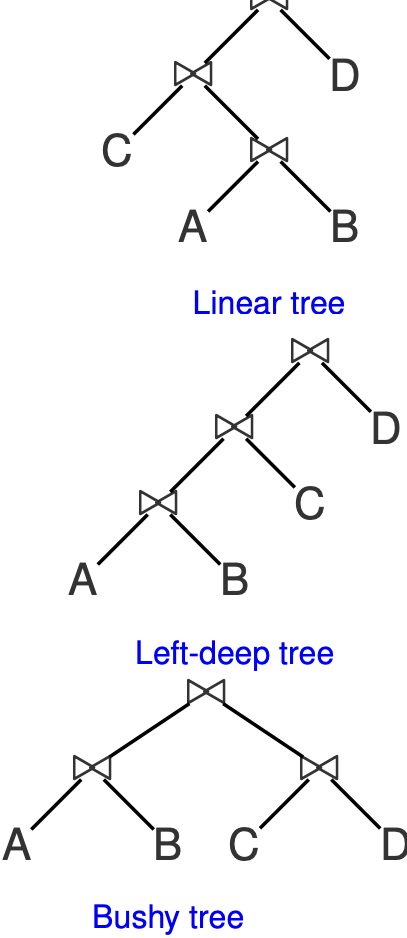
\includegraphics[width=\columnwidth, height=3.5cm]{images/typesofqueryplans.png}
\end{minipage}

\textbf{Relationships of Schedules:} “Serial” is a proper subset of “Strict”
\includegraphics*[width=8.5cm, height=2.5cm]{images/relationshipsofschedules.png}

\subsubsubsection{System R Optimizer}
\begin{itemize}
    \item Uses heuristics to prune search space:
    \begin{itemize}
        \item Enumerates only left-deep query plans
        \item Avoids cross-product query plans
        \item Considers early $\sigma$ (selections) \& $\pi$ (projections)
    \end{itemize}
    \item Uses enhanced dynamic programming approach that considers sort order of
    query plan's output
    \begin{itemize}
        \item Maintains $\text{optPlan}(S_i, o_i)$ instead of $\text{optPlan}(S_i)$
        \item $o_i$ captures the sort order of output produced by query plan w.r.t. $S_i$
        \item $o_i = \begin{cases} 
            \text{null} & \text{if output is unordered} \\
            \langle A_1, \ldots, A_k \rangle & \text{sequence of attributes}
            \end{cases}$
        \item $\text{optPlan}(S_i, o_i) =$ cheapest query plan for relations $S_i$ with output ordered by $o_i$ if $o_i \neq \text{null}$
    \end{itemize}
\end{itemize}

\subsubsubsection{Cost Estimation of Query Plans}
\begin{enumerate}
    \item What is eval cost of each operation? size of input, avail buffer pages/index etc.
    \item What is the output size of each operation?
    \item How to estimate?: with the following assumptions:
        \begin{enumerate}
            \item Uniformity: uniform distribution of attribute values
            \item Independence: independent distribution of values in different attributes
            \item Inclusion: For $R \bowtie_{R.A=S.B} S$, if $||\pi_A(R)|| \leq ||\pi_B(S)||$, then $\pi_A(R) \subseteq \pi_B(S)$
        \end{enumerate}
        % \item Database statistics: relation ardinality, number of distinct values in each column, highest/lowest values in each column, frequency of values, column group statistics etc.
\end{enumerate}

\subsubsubsection{Size estimation}
\begin{itemize}
    \item \textbf{Reduction factor} (a.k.a \textcolor{red}{selectivity factor}) of a term $t_i$ (denoted by \textcolor{red}{$rf(t_i)$}) is the fraction of tuples in $e$ that satisfy $t_i$; i.e., $rf(t_i) = \frac{||\sigma_{t_i}(e)||}{||e||}$
    \item Assuming terms in $p$ are statistically independent: $||q|| \approx ||e|| \times \prod_{i=1}^{n} rf(t_i)$
\end{itemize}

\subsubsubsection{Join Selectivity}
\begin{itemize}
    \item \textbf{\textcolor{red}{Join selectivity factor}} = selectivity factor for join predicates
    \begin{itemize}
        \item Consider query Q: SELECT * FROM R JOIN S ON R.A = S.B
        \item $rf(R.A = S.B) = \frac{||R \bowtie_{R.A=S.B} S||}{||R|| \times ||S||}$
    \end{itemize}
    \item \textbf{\textcolor{red}{Inclusion assumption}}: Consider $R \bowtie_{R.A=S.B} S$
    \begin{itemize}
        \item If $||\pi_A(R)|| \leq ||\pi_B(S)||$, then $\pi_A(R) \subseteq \pi_B(S)$
    \end{itemize}
    \item \textbf{Join selectivity estimation}:
    \begin{itemize}
        \item Assume $||\pi_A(R)|| \leq ||\pi_B(S)||$
        \item By inclusion assumption, every R-tuple joins with some S-tuple
        \item By uniformity assumption, there are $\frac{||S||}{||\pi_B(S)||}$ S-tuples corresponding to each S.B value
        \item Therefore, each R-tuple joins with $\frac{||S||}{||\pi_B(S)||}$ S-tuples
        \item Thus, $||Q|| \approx ||R|| \times \frac{||S||}{||\pi_B(S)||}$
    \end{itemize}
    \item $rf(R.A = S.B) \approx \frac{1}{\max\{||\pi_A(R)||, ||\pi_B(S)||\}}$
\end{itemize}

\subsubsubsection{Estimation using Histograms}
\begin{itemize}
    \item \textit{histogram} = statistical info maintained by DBMS to estimate data distribution
    \begin{itemize}
        \item Partition attribute’s domain into sub-ranges called buckets
        \item Assume value distribution within each bucket is uniform
    \end{itemize}
    \item Types of histograms:
    \begin{itemize}
        \item \textbf{Equiwidth histograms}: Each bucket has (almost) equal number of values
        \item \textbf{Equidepth histograms}: Each bucket has (almost) equal number of tuples, sub-ranges of adjacent buckets might overlap
    \end{itemize}
\end{itemize}

\subsubsubsection{Improved Histogram Estimation with MCV | Most Comon Values}
\begin{itemize}
    \item Separately keep track of the frequencies of the top-$k$ most common values and exclude MCV from histogram’s buckets
\end{itemize}
\includegraphics*[width=8.5cm, height=2.3cm]{images/mcv.png}

\subsection{7. Transaction Management}
\begin{enumerate}
    \item \textcolor{red}{Atomicity}: Either all or none of the actions in transaction happen
    \item \textcolor{red}{Consistency}: If each txn \& DB starts consistent, DB ends up consistent
    \item \textcolor{red}{Isolation}: Execution of one transaction is isolated from other transactions
    \item \textcolor{red}{Durability}: If a transaction commits, its effects persist
\end{enumerate}
\textcolor{blue}{concurrency control manager} $\rightarrow$ isolation, \textcolor{blue}{recovery manager} $\rightarrow$ atomicity + durability

\textbf{Transactions} | Each Xact \underline{must end with either} a commit or an abort action
\begin{itemize}
    \item A transaction (Xact) $T_i$ can be viewed as a sequence of \textcolor{red}{actions}:
    \begin{itemize}
        \item $R_i(O)$ = $T_i$ reads an object O
        \begin{itemize}
            \item $R_i(O, v)$ = $T_i$ reads an object O whose value is $v$
        \end{itemize}
        \item $W_i(O)$ = $T_i$ writes an object O
        \begin{itemize}
            \item $W_i(O, v)$ = $T_i$ writes an object O with a value of $v$
        \end{itemize}
        \item \textcolor{blue}{Commit$_i$} (or $C_i$) = $T_i$ terminates successfully
        \item \textcolor{blue}{Abort$_i$} (or $A_i$) = $T_i$ terminates unsuccessfully
    \end{itemize}
    \item A Xact is an \textcolor{red}{active Xact} if it is still in progress (i.e., has not yet terminated); otherwise, it is a \textcolor{red}{completed Xact} (i.e., committed or aborted)
\end{itemize}

\subsubsubsection{Transactions Schedules}
\begin{itemize}
    \item \textcolor{red}{Schedule} = a list of actions from a set of Xacts, where the order of the actions within each Xact is preserved
    \item \textbf{Example:} Consider two Xacts $T_1$ and $T_2$:
    % \begin{itemize}
    %     \item $T_1$: $\textcolor{blue}{R_1(A)}$, $\textcolor{blue}{W_1(A)}$, $\textcolor{blue}{R_1(B)}$, $\textcolor{blue}{W_1(B)}$, $\textcolor{blue}{\text{Commit}_1}$
    %     \item $T_2$: $\textcolor{red}{R_2(A)}$, $\textcolor{red}{W_2(A)}$, $\textcolor{red}{R_2(B)}$, $\textcolor{red}{W_2(B)}$, $\textcolor{red}{\text{Commit}_2}$
    % \end{itemize}
    % \item Some schedules of $T_1$ and $T_2$:
    % \begin{itemize}
    %     \item $S_1$: $\textcolor{blue}{R_1(A)}$, $\textcolor{blue}{W_1(A)}$, $\textcolor{blue}{R_1(B)}$, $\textcolor{blue}{W_1(B)}$, $\textcolor{blue}{\text{Commit}_1}$, $\textcolor{red}{R_2(A)}$, $\textcolor{red}{W_2(A)}$, $\textcolor{red}{R_2(B)}$, $\textcolor{red}{W_2(B)}$, $\textcolor{red}{\text{Commit}_2}$
    %     \item $S_2$: $\textcolor{red}{R_2(A)}$, $\textcolor{red}{W_2(A)}$, $\textcolor{red}{R_2(B)}$, $\textcolor{red}{W_2(B)}$, $\textcolor{red}{\text{Commit}_2}$, $\textcolor{blue}{R_1(A)}$, $\textcolor{blue}{W_1(A)}$, $\textcolor{blue}{R_1(B)}$, $\textcolor{blue}{W_1(B)}$, $\textcolor{blue}{\text{Commit}_1}$
    %     \item $S_3$: $\textcolor{blue}{R_1(A)}$, $\textcolor{blue}{W_1(A)}$, $\textcolor{red}{R_2(A)}$, $\textcolor{red}{W_2(A)}$, $\textcolor{blue}{R_1(B)}$, $\textcolor{blue}{W_1(B)}$, $\textcolor{blue}{\text{Commit}_1}$, $\textcolor{red}{R_2(B)}$, $\textcolor{red}{W_2(B)}$, $\textcolor{red}{\text{Commit}_2}$
    % \end{itemize}
    \item A \textcolor{red}{serial schedule} is a schedule where the actions of Xacts are not interleaved
\end{itemize}

\subsubsubsection{Read From \& Final Write | Dirty Read \& Dirty Write}
\begin{itemize}
    \item We say that $T_j$ \textcolor{blue}{reads $O$ from $T_i$} in a schedule $S$ if the last write action on $O$ before $R_j(O)$ in $S$ is $W_i(O)$
    \item We say that $T_j$ \textcolor{blue}{reads from $T_i$} if $T_j$ has read some object from $T_i$
    \item We say that $T_i$ \textcolor{blue}{performs the final write on $O$} in a schedule $S$ if the last write action on $O$ in $S$ is $W_i(O)$
    % \item \textbf{Example:} Consider the following schedule:
    % \begin{itemize}
    %     \item $\textcolor{blue}{R_1(A)}$, $\textcolor{blue}{W_1(A)}$, $\textcolor{red}{R_2(A)}$, $\textcolor{red}{W_2(A)}$, $\textcolor{blue}{R_1(B)}$, $\textcolor{blue}{W_1(B)}$, $\textcolor{blue}{\text{Commit}_1}$, $\textcolor{red}{R_2(B)}$, $\textcolor{red}{W_2(B)}$, $\textcolor{red}{\text{Commit}_2}$
    %     \item $T_1$ reads $A$ from the initial database (or $T_1$ reads A from $T_0$)
    %         \begin{itemize}
    %             \item Assume that initial database was created by a \textcolor{blue}{dummy Xact $T_0$}
    %         \end{itemize}
    %     \item $T_2$ reads $A$ from $T_1$, $T_1$ reads $B$ from $T_0$, $T_2$ reads $B$ from $T_1$
    %     \item $T_2$ performs the final write on $A$, $T_2$ performs the final write on $B$
    % \end{itemize}
    \item \textcolor{red}{dirty read} if the read value was produced by an active transaction
    \item \textcolor{red}{dirty write} if the overwritten value of O was produced by an active transaction
\end{itemize}

% \subsubsubsection{Dirty Read \& Dirty Write}
% \begin{itemize}
%     \item A read on an object is call a \textcolor{red}{dirty read} if the read value was produced by an active transaction
%     \begin{itemize}
%         \item Consider the schedule: $W_1(x)$, $R_2(x)$, $\text{Commit}_1$, $R_3(x)$
%         \item $R_2(x)$ is a dirty read, $R_3(x)$ is not a dirty read
%     \end{itemize}
%     \item A write on object O is call a \textcolor{red}{dirty write} if the overwritten value of O was produced by an active transaction
%     \begin{itemize}
%         \item Consider the schedule: $W_1(x)$, $W_2(x)$, $\text{Commit}_1$, $W_3(x)$
%         \item $W_2(x)$ is a dirty write, $W_1(x)$ and $W_3(x)$ are not dirty writes
%     \end{itemize}
% \end{itemize}

\textbf{Correctness of Interleaved Xact Executions:} An interleaved Xact execution schedule is \textbf{correct} if it is ``equivalent'' to some serial schedule over the same set of Xacts
% \begin{tabular}{|p{0.25\linewidth}|p{0.25\linewidth}|p{0.25\linewidth}|}
%     \hline
%     Execution & \multicolumn{2}{c|}{Serial Schedules} \\
%     \cline{2-3}
%     Schedule & $S_1$ & $S_2$ \\
%     \hline
%     $\textcolor{red}{R_1(x,400)}$ & $\textcolor{red}{R_1(x,400)}$ & $\textcolor{blue}{R_2(y,100)}$ \\
%     $\textcolor{red}{R_1(y,100)}$ & $\textcolor{red}{R_1(y,100)}$ & $\textcolor{blue}{R_2(x,400)}$ \\
%     $\textcolor{red}{W_1(y,200)}$ & $\textcolor{red}{W_1(y,200)}$ & $\textcolor{blue}{W_2(x,500)}$ \\
%     $\textcolor{blue}{R_2(y,200)}$ & $\textcolor{red}{W_1(x,300)}$ & $\textcolor{blue}{W_2(y,0)}$ \\
%     $\textcolor{blue}{R_2(x,400)}$ & $\textcolor{red}{Commit_1}$ & $\textcolor{blue}{Commit_2}$ \\
%     $\textcolor{red}{W_1(x,300)}$ & $\textcolor{blue}{R_2(y,200)}$ & $\textcolor{red}{R_1(x,500)}$ \\
%     $\textcolor{red}{Commit_1}$ & $\textcolor{blue}{R_2(x,300)}$ & $\textcolor{red}{R_1(y,0)}$ \\
%     $\textcolor{blue}{W_2(x,500)}$ & $\textcolor{blue}{W_2(x,400)}$ & $\textcolor{red}{W_1(y,100)}$ \\
%     $\textcolor{blue}{W_2(y,100)}$ & $\textcolor{blue}{W_2(y,100)}$ & $\textcolor{red}{W_1(x,400)}$ \\
%     $\textcolor{blue}{Commit_2}$ & $\textcolor{blue}{Commit_2}$ & $\textcolor{red}{Commit_1}$ \\
%     \hline
% \end{tabular}


\textbf{View Serializable Schedule:} if view eqv to some serial schedule over same set of txns
\begin{itemize}
    \item Two schedules $S$ and $S'$ (over the same set of Xacts) are \textbf{view equivalent} (denoted by $S \equiv_v S'$) if they satisfy all the following conditions:
    \begin{enumerate}
        \item If $T_i$ reads $A$ from $T_j$ in $S$, then $T_i$ must also read $A$ from $T_j$ in $S'$
        \item For each data object $A$, the Xact (if any) that performs the final write on $A$ in $S$ must also perform the final write on $A$ in $S'$
    \end{enumerate}
\end{itemize}

\textbf{Testing for View Serializability | \underline{Check WR and Final Write}} \\ 
\hl{\textbf{Theorem 1:} S is VSS iff there exists some VSG(S) corresponding to S that is acyclic}
\begin{itemize}
    \item A \textcolor{red}{\textbf{view serializability graph}} for a schedule $S$ (denoted by \textcolor{red}{$VSG(S)$}) is a directed graph $VSG(S) = (V, E)$ such that the nodes $V$ represent Xacts \& the edges $E$ represent precedence relations among Xacts:
    \begin{enumerate}
        \item If $T_i$ reads from $T_j$, then $(T_j, T_i) \in E$
        \item If both $T_i$ \& $T_j$ update the same object $O$ \& $T_j$ performs the final write on $O$, then $(T_i, T_j) \in E$
        \item If $T_i$ read some object $O$ from $T_k$ \& $T_j$ update object $O$, then either $(T_i, T_k) \in E$ or $(T_j, T_i) \in E$
    \end{enumerate}
    \item Due to (c), there could be multiple VSG(S) corresponding to S
    \item 2 actions on same $O$ conflict if $\geq 1$ is write action OR actions are from diff Xacts
\end{itemize}

\subsubsubsection{Anomalies with Interleaved Xact Executions}
\begin{itemize}
    \item Anomalies can arise due to conflicting actions:
    \begin{enumerate}
        \item \textcolor{red}{Dirty read problem} (due to WR conflicts)
        \begin{itemize}
            \item[$\star$] $T_2$ reads an object that has been modified by $T_1$ and $T_1$ has not yet committed (i.e., $T_2$'s read is a dirty read)
            \item[$\star$] $T_2$ could see an inconsistent DB state!
        \end{itemize}
        \item \textcolor{red}{Unrepeatable read problem} (due to RW conflicts)
        \begin{itemize}
            \item[$\star$] $T_2$ updates an object that $T_1$ has previously read and $T_2$ commits while $T_1$ is still in progress
            \item[$\star$] $T_1$ could get a different value if it reads the object again!
        \end{itemize}
        \item \textcolor{red}{Lost update problem} (due to WW conflicts)
        \begin{itemize}
            \item[$\star$] $T_2$ overwrites the value of an object that has been modified by $T_1$ while $T_1$ is still in progress (i.e., $T_2$'s write is a dirty write)
            \item[$\star$] $T_1$'s update is lost!
        \end{itemize}
    \end{enumerate}
\end{itemize}

\subsubsubsection{Conflict Serializable Schedules}
\begin{itemize}
    \item Two schedules $S$ \& $S'$ (over the same set of Xacts) are said to be \textcolor{red}{conflict equivalent} (denoted by $S \equiv_c S'$) if they order every pair of conflicting actions of two committed Xacts in the same way
    \item A schedule is a \textcolor{red}{\textbf{conflict serializable schedule (CSS)}} if
    it is conflict equivalent to a serial schedule over the
    same set of Xacts
\end{itemize}

\textbf{Testing for Conflict Serializability | \underline{Check WR, RW, WW}} \\ 
\begin{itemize}
    \item A \textcolor{red}{conflict serializability graph} (check $R\rightarrow W$ and $W\rightarrow W$ edges) for a schedule $S$ (denoted by $CSG(S)$) is a directed graph $CSG(S) = (V,E)$ s.t.
    \begin{itemize}
        \item[$\triangleright$] $V$ contains a node for each Xact in $S$
        \item[$\triangleright$] $E$ contains $(T_i, T_j)$ if action in $T_i$ precedes \& conflicts w/ 1 of $T_j$'s actions
    \end{itemize}
        % \item \textbf{Example:} Conflict serializability graph for schedule\\
        % $R_1(A)$, $W_2(A)$, $\text{Commit}_2$, $W_1(A)$, $\text{Commit}_1$, $W_3(A)$, $\text{Commit}_3$
        % \columnbreak
        % \includegraphics*[width=4.2cm, height=2cm]{images/css.png}
    \item \hl{\textbf{Theorem 2:} A schedule is CSS iff its conflict serializability graph is \textit{acyclic}}
    \item \hl{\textbf{Theorem 3:} A schedule that is CSS is also view serializable}
\end{itemize}

\subsubsubsection{Blind Writes}
\begin{itemize}
    \item W on object $O$ by $T_i$ is called a \textcolor{red}{blind write} if $T_i$ did not read $O$ prior to the write
    \item \hl{\textbf{Theorem 4:} If $S$ is VSS and $S$ has no blind writes, then $S$ is also CSS}
\end{itemize}

\subsubsubsection{Cascading Aborts}
\begin{itemize}
    \item For correctness, if $T_i$ has read from $T_j$, then $T_i$ must abort if $T_j$ aborts
    \begin{itemize}
        \item Consider the schedule: $W_1(x)$, $R_2(x)$, $W_2(y)$, $\text{Abort}_1$
        \item $T_2$ must abort since it read from $T_1$ which aborted
    \end{itemize}
    \item We say that $T_1$'s abort is \textcolor{blue}{cascaded} to $T_2$
    \item Recursive aborting process is known as \textcolor{red}{cascading abort}
    % \item \textbf{Example:}
    % \begin{multicols}{2}
    %     \begin{tabular}{ll}
    %         $T_1$ & $T_2$ \\
    %         \hline
    %         $W_1(x)$ & \\
    %         & $R_2(x)$ \\
    %         & $W_2(y)$ \\
    %         $\text{Abort}_1$ & \\
    %     \end{tabular}
    %     \begin{tabular}{ll}
    %         $T_1$ & $T_2$ \\
    %         \hline
    %         $W_1(x)$ & \\
    %         & $R_2(x)$ \\
    %         & $W_2(y)$ \\
    %         & $\text{Abort}_2$ \\
    %     \end{tabular}
    % \end{multicols}
\end{itemize}

\textbf{Recoverable Schedules}
\begin{multicols}{3}
    \begin{itemize}
        \item A schedule $S$ is said to be a \textcolor{red}{recoverable schedule} if for every Xact $T$ that commits in $S$, $T$ must commit after $T'$ if $T$ reads from $T'$
        \item This is a \textcolor{blue}{non-recoverable schedule} because $T_2$ commits before $T_1$ commits even though $T_2$ reads from $T_1$
    \end{itemize}
    \columnbreak
    \begin{tabular}{ll}
        $T_1$ & $T_2$ \\
        \hline
        $W_1(x)$ & \\
        & $R_2(x)$ \\
        & $W_2(y)$ \\
        & $\text{Commit}_2$ \\
    \end{tabular}
\end{multicols} 

\begin{itemize}
    \item[] \hspace*{-0.7em}\textbf{Cascadeless Schedules}
    \begin{multicols}{2}
    \item \textbf{Undesirable}: cost of bookkeeping to identify \& performance penalty incurred
    \item To avoid cascading aborts (or to be \textcolor{red}{cascadeless}), DBMS must permit reads only from committed Xacts
    \item A schedule $S$ is a \textcolor{red}{cascadeless schedule} if there is no dirty read in $S$
    \columnbreak
    \item \hl{\textbf{Theorem 5:} A cascadeless schedule is also a recoverable schedule}
    \begin{lstlisting}[basicstyle=\tiny\ttfamily, aboveskip=0pt, belowskip=0pt, backgroundcolor=\color{lightgray}]
for every Read Rj(X)
  if there exists a Wi(X) before it  
    if Commit(Ti) is after Rj
      return NOT cascadeless
return cascadeless
\end{lstlisting}
\end{multicols}
\end{itemize}

\textbf{Recovery using Before-Images}
\begin{itemize}
    \item An efficient approach to undo the actions of aborted Xacts is to restore before-images for writes
    \item We use $W_i(x,v)$ to denote that $T_i$ updates the value of object $x$ to $v$
    \item \textbf{Example:} Consider the following schedule $S$:
    \begin{itemize}
        \item $W_1(A,100)$, $W_2(A,200)$, $\text{Abort}_2$
        \item Assume that the initial value of $A$ is 50
        \item Before performing $W_1(A,100)$, its before-image ``$A=50$'' is logged
        \item Before performing $W_2(A,200)$, its before-image ``$A=100$'' is logged
        \item To recover from $\text{Abort}_2$, $W_2(A,200)$ is undone by restoring the before-image of $A$ (i.e., the value of $A$ is restored to 100)
    \end{itemize}
    \item However, before-image recovery doesn’t always work!
    \item $W_1(A,100)$, $W_2(A,200)$, $Abort_1$
    \item Here, undoing $W_1(A,100)$ by restoring A to its before-image of 50 is incorrect!
\end{itemize}

\subsubsubsection{Strict Schedules}
\begin{itemize}
    % \item To enable the use of before-images for recovery, we use strict schedules
    \item A schedule $S$ is a \textcolor{red}{strict schedule} if there is no dirty read and no dirty write in $S$
    \begin{multicols}{2}
        \begin{lstlisting}[basicstyle=\tiny\ttfamily, aboveskip=0pt, belowskip=0pt, backgroundcolor=\color{lightgray}]
for every Read Rj(X) or Write Wj(X)
  if there exists a Wi(X) before it
    if Commit(Ti) is after Rj or Wj
      return NOT strict
return strict
    \end{lstlisting}
    \item \textbf{Example:}
    \begin{itemize} 
        \item $S$: $W_1(A)$, $W_2(A)$, $\text{Abort}_2$, $S'$: $W_1(A)$, $W_2(A)$, $\text{Abort}_1$
        \item Both $S$ and $S'$ are not strict schedules
    \end{itemize}
\end{multicols}
    \item \textbf{Performance Tradeoff:} recovery (w/ before-images) more efficient but concurrent executions become more restrictive
    \item \hl{\textbf{Theorem 6:} A strict schedule is also a cascadeless schedule}
\end{itemize}

\subsection{8. Concurrency Control}
% \subsubsubsection{Transaction Scheduler}
% \begin{itemize}
%   \item For each input action (read, write, commit, abort) to the scheduler, the scheduler performs one of the following:
%   \begin{itemize}
%     \item output the action to the schedule,
%     \item postpone the action by blocking the transaction, or
%     \item reject the action and abort the transaction
%   \end{itemize}
% \end{itemize}

\subsubsubsection{Lock-Based Concurrency Control}
\begin{itemize}
  \item Each Xact needs to request for an \textit{appropriate lock} before it can access the object
  \item \textbf{Locking modes:}
  \begin{itemize}
    \item \textcolor{blue}{Shared (S)} locks for reading objects OR \textcolor{blue}{Exclusive (X)} locks for writing objects
  \end{itemize}
\end{itemize}

% \begin{multicols}{2}
% \begin{tabular}{|c|c|c|c|}
%     \hline
%     \rowcolor{lightgray}
%     \tiny \diagbox[width=14em]{Lock Requested}{Lock Held} & \tiny - & \tiny S & \tiny X \\
%     \hline
%     S & $\checkmark$ & $\checkmark$ & $\times$ \\
%     \hline
%     X & $\checkmark$ & $\times$ & $\times$ \\
%     \hline
% \end{tabular}

% \begin{itemize}
%   \item[$\checkmark$:] Compatible (Lock request is granted)
%   \item[$\times$:] Incompatible (Lock request is blocked)
% \end{itemize}
% \end{multicols}

\begin{itemize}
    % \item To \textcolor{blue}{read} an object $O$, a Xact must request for a shared/exclusive lock on $O$
    % \item To \textcolor{blue}{update} an object $O$, a Xact must request for an exclusive lock on $O$
    % \item A \textcolor{blue}{lock request is granted} on $O$ if the requesting lock mode is compatible with the lock modes of existing locks on $O$
    \item If $T$'s \textcolor{blue}{lock request is not granted} on $O$, $T$ becomes blocked; its execution is suspended \& $T$ is added to $O$'s \textcolor{red}{request queue}
    \item When a \textcolor{blue}{lock is released} on $O$, the lock manager checks the request of the first Xact $T$ in the request queue for $O$. If $T$'s request can be granted, $T$ acquires its lock on $O$ and resumes execution after its removal from the queue
    \item When a Xact \textcolor{blue}{commits/aborts}, all its locks are released \& $T$ is removed from any request queue it is in
\end{itemize}

% \textbf{Notations:}
% \begin{itemize}
%     \item \textcolor{blue}{$S_i(O)$}: Xact $T_i$ requests S-lock on object $O$
%     \item \textcolor{blue}{$X_i(O)$}: Xact $T_i$ requests X-lock on object $O$
%     \item \textcolor{blue}{$U_i(O)$}: Xact $T_i$ releases lock on object $O$
% \end{itemize}

\subsubsubsection{Two Phase Locking (2PL) Protocol}
\begin{itemize}
    \item \textbf{2PL Protocol:}
    \begin{enumerate}
        \item To read an object $O$, a Xact must hold a S-lock or X-lock on $O$
        \item To write to an object $O$, a Xact must hold a X-lock on $O$
        \item Once a Xact releases a lock, the Xact can't request any more locks
    \end{enumerate}
    \item Xacts using 2PL can be characterized into two phases:
    \begin{itemize}
        \item \textcolor{blue}{Growing}: before releasing 1\textsuperscript{st} lock | \textcolor{blue}{Shrinking}: after releasing 1\textsuperscript{st} lock
    \end{itemize}
    \item \hl{\textbf{Theorem 1:} 2PL schedules are conflict serializable}
    \item \textbf{Strict 2PL Protocol:}
    \begin{enumerate}
        \item To read an object $O$, a Xact must hold a S-lock or X-lock on $O$
        \item To write to an object $O$, a Xact must hold a X-lock on $O$
        \item \textcolor{blue}{A Xact must hold on to locks until Xact commits or aborts}
    \end{enumerate}
    \item \hl{\textbf{Theorem 2:} Strict 2PL schedules are strict \& conflict serializable}
\end{itemize}

\textbf{Deadlock}: cycle of Xacts \textit{waiting for locks to be released} by each other
\begin{itemize}
    \item \textbf{How to Detect Deadlocks?}
    \begin{multicols}{2}
        \begin{itemize}
            \item \textbf{Waits-for graph (WFG)}
            \begin{itemize}
                \item Nodes represent active Xacts
                \item Add an edge $T_i \rightarrow T_j$ if $T_i$ is waiting for $T_j$ to release a lock
            \end{itemize}
            \item \textbf{Lock manager}
            \begin{itemize}
                \item adds an edge when it queues a lock request, updates edges when it grants a lock request
            \end{itemize}
            \item Deadlock detected if WFG has cycle, break by aborting a Xact in cycle
            \item Alternative to WFG: timeout mechanism
        \end{itemize}
    \end{multicols}
    \item \textbf{How to Prevent Deadlocks?}
    \begin{itemize}
        \item Assume older Xacts have higher priority than younger Xacts
        \begin{itemize}
            \item Each Xact is assigned a timestamp when it starts, older txn has smaller
        \end{itemize}
        \item Suppose $T_i$ requests for a lock that conflicts with a lock held by $T_j$
        \begin{itemize}
            \item \textcolor{blue}{Wait-die policy}:
            \begin{itemize}
                \item non-preemptive: only a Xact requesting for a lock can get aborted
                \item a younger Xact may \underline{get repeatedly aborted} 
                \item a Xact that has all the locks it needs is never aborted
            \end{itemize}
            \item \textcolor{blue}{Wound-wait policy}: preemptive, higher-priority never wait for lower-priority
            \item To avoid starvation, a restarted Xact must use its \textit{\underline{original timestamp!}}
        \end{itemize}
            \tiny
            \begin{tabular}{|c|c|c|}
                \hline
                \rowcolor{lightgray}
                Prevention Policy & $T_i$ has higher priority & $T_i$ has lower priority \\
                \hline
                Wait-die & $T_i$ waits for $T_j$ & $T_i$ aborts \\
                \hline
                Wound-wait & $T_j$ aborts & $T_i$ waits for $T_j$ \\
                \hline
            \end{tabular}
    \end{itemize}
\end{itemize}

\subsubsubsection{Lock Conversions}
\begin{itemize}
    % \item Consider two Xacts:
    % \begin{itemize}
    %     \item $\textcolor{blue}{T_1: } \textcolor{blue}{R_1(A)}, \textcolor{blue}{R_1(B)}, \textcolor{blue}{W_1(A)}$
    %     \item $\textcolor{red}{T_2: } \textcolor{red}{R_2(A)}, \textcolor{red}{R_2(B)}$
    % \end{itemize}
    % \item Since $\textcolor{blue}{T_1}$ needs to update $A$, $\textcolor{blue}{T_1}$ requires an exclusive lock on $A$
    % \item All possible schedules are serial
    % \begin{itemize}
    %     \item $S_1$: $\textcolor{blue}{X_1(A)}, \textcolor{blue}{R_1(A)}, \textcolor{blue}{S_1(B)}, \textcolor{blue}{R_1(B)}, \textcolor{blue}{W_1(A)}, \textcolor{blue}{U_1(A)}, \textcolor{blue}{U_1(B)}, \textcolor{red}{S_2(A)}$, $\textcolor{red}{R_2(A)}, \textcolor{red}{S_2(B)}, \textcolor{red}{R_2(B)}$
    %     \item $S_2$: $\textcolor{red}{S_2(A)}, \textcolor{red}{R_2(A)}, \textcolor{red}{S_2(B)}, \textcolor{red}{R_2(B)}, \textcolor{red}{U_2(A)}, \textcolor{red}{U_2(B)}$, $\textcolor{blue}{X_1(A)}, \textcolor{blue}{R_1(A)}, \textcolor{blue}{S_1(B)}, \textcolor{blue}{R_1(B)}, \textcolor{blue}{W_1(A)}, \textcolor{blue}{U_1(A)}, \textcolor{blue}{U_1(B)}$
    % \end{itemize}
    \item Increase concurrency by allowing $\textcolor{blue}{\text{lock conversions}}$
    \item Two types of lock conversions:
    \begin{itemize}
        \item $\textcolor{red}{UG_i(A)}$: $T_i$ requests to upgrade its S-lock on object $A$ to X-lock
        \item $\textcolor{red}{DG_i(A)}$: $T_i$ requests to downgrade its X-lock on object $A$ to S-lock
    \end{itemize}
\end{itemize}

\subsubsubsection{2PL with Lock Upgrades}
\begin{itemize}
    \item \textbf{2PL with lock upgrades}
    \begin{itemize}
        \item To perform $R_i(O)$, $T_i$ must be holding a $S / X$ lock on $O$. If not, $T_i$ requests for a $S$ on $O$ (i.e., $S_i(O)$)
        \item To perform $W_i(O)$, $T_i$ must be holding an exclusive lock on $O$. If not,
        \begin{itemize}
            \item[$\triangleright$] If $T_i$ is \textit{holding a shared lock} on $O$, $T_i$ requests for a $UG_i(O)$
            \item[$\triangleright$] If $T_i$ is \textit{not holding any lock} on $O$, $T_i$ requests for a $X_i(O)$
        \end{itemize}
    \end{itemize}
\end{itemize}

\begin{itemize}
    \item $UG_i(O)$ is allowed only in the \textbf{growing phase} (i.e., $T_i$ has not released any lock)
    \item $UG_i(O)$ is blocked if another Xact is holding a shared lock on $O$
    \item If $UG_i(O)$ is granted, $S_i(O)$ becomes $X_i(O)$
    % \item Consider again previous example with two Xacts:
    % \begin{itemize}
    %     \item \textcolor{blue}{$T_1$}: \textcolor{blue}{$R_1(A)$}, \textcolor{blue}{$R_1(B)$}, \textcolor{blue}{$W_1(A)$}
    %     \item \textcolor{red}{$T_2$}: \textcolor{red}{$R_2(A)$}, \textcolor{red}{$R_2(B)$}
    % \end{itemize}
    % \item Possible schedules using 2PL without lock upgrades: $S_1$, $S_2$
    % \item Possible schedules using 2PL with lock upgrades: $S_1$, $S_2$, $S_3$, $S_4$, $S_5$
    % \begin{itemize}
    %     \item $S_1$: $\textcolor{blue}{X_1(A)}$, $\textcolor{blue}{R_1(A)}$, $\textcolor{blue}{S_1(B)}$, $\textcolor{blue}{R_1(B)}$, $\textcolor{blue}{W_1(A)}$, $\textcolor{blue}{U_1(A)}$, $\textcolor{blue}{U_1(B)}$, $\textcolor{red}{S_2(A)}$, $\textcolor{red}{R_2(A)}$, $\textcolor{red}{S_2(B)}$, $\textcolor{red}{R_2(B)}$, $\textcolor{red}{U_2(A)}$, $\textcolor{red}{U_2(B)}$
    %     \item $S_2$: $\textcolor{red}{S_2(A)}$, $\textcolor{red}{R_2(A)}$, $\textcolor{red}{S_2(B)}$, $\textcolor{red}{R_2(B)}$, $\textcolor{red}{U_2(A)}$, $\textcolor{red}{U_2(B)}$, $\textcolor{blue}{X_1(A)}$, $\textcolor{blue}{R_1(A)}$, $\textcolor{blue}{S_1(B)}$, $\textcolor{blue}{R_1(B)}$, $\textcolor{blue}{W_1(A)}$, $\textcolor{blue}{U_1(A)}$, $\textcolor{blue}{U_1(B)}$
    %     \item $S_3$: $\textcolor{blue}{S_1(A)}$, $\textcolor{blue}{R_1(A)}$, $\textcolor{blue}{S_1(B)}$, $\textcolor{blue}{R_1(B)}$, $\textcolor{red}{S_2(A)}$, $\textcolor{red}{R_2(A)}$, $\textcolor{red}{S_2(B)}$, $\textcolor{red}{R_2(B)}$, $\textcolor{red}{U_2(A)}$, $\textcolor{red}{U_2(B)}$, $\textcolor{blue}{UG_1(A)}$, $\textcolor{blue}{W_1(A)}$, $\textcolor{blue}{U_1(A)}$, $\textcolor{blue}{U_1(B)}$
    %     \item $S_4$: $\textcolor{blue}{S_1(A)}$, $\textcolor{blue}{R_1(A)}$, $\textcolor{blue}{S_1(B)}$, $\textcolor{blue}{R_1(B)}$, $\textcolor{red}{S_2(A)}$, $\textcolor{red}{R_2(A)}$, $\textcolor{red}{S_2(B)}$, $\textcolor{red}{R_2(B)}$, $\textcolor{blue}{UG_1(A)}$, $\textcolor{blue}{W_1(A)}$, $\textcolor{blue}{U_1(A)}$, $\textcolor{blue}{U_1(B)}$, $\textcolor{red}{U_2(A)}$, $\textcolor{red}{U_2(B)}$
    %     \item $S_5$: $\textcolor{blue}{S_1(A)}$, $\textcolor{blue}{R_1(A)}$, $\textcolor{blue}{S_1(B)}$, $\textcolor{blue}{R_1(B)}$, $\textcolor{blue}{UG_1(A)}$, $\textcolor{blue}{W_1(A)}$, $\textcolor{blue}{U_1(A)}$, $\textcolor{blue}{U_1(B)}$, $\textcolor{red}{S_2(A)}$, $\textcolor{red}{R_2(A)}$, $\textcolor{red}{S_2(B)}$, $\textcolor{red}{R_2(B)}$, $\textcolor{red}{U_2(A)}$, $\textcolor{red}{U_2(B)}$
    % \end{itemize}
\end{itemize}

\subsubsubsection{Performance of Locking}
\begin{itemize}
    \item Resolve Xact conflicts by using \textcolor{red}{blocking} and \textcolor{red}{aborting} mechanisms
    \item Blocking causes delays in other waiting Xacts
    \item Aborting and restarting a Xact wastes work done by Xact
    \item How to increase system throughput?
    \begin{enumerate}
        \item Reduce the locking granularity | Reduce the time a lock is held
        \item Reduce hot spots | a DB object that is \textit{frequently accessed and modified}
    \end{enumerate}
\end{itemize}

\subsubsubsection{Phantom read problem}
A transaction \textbf{re-executes a query} and sees new rows (phantoms) that were not there before
\begin{itemize}
    \item Phantom problem can be prevented by \textcolor{red}{predicate locking}
    \begin{itemize}
        \item Xact 1 is granted a shared lock on the predicate $balance > 1000$
        \item Xact 2’s request for an exclusive lock on predicate $balance = 3000$ is blocked
        \item e.g., T1 reads all accounts with $balance > 1000$; T2 inserts account with $balance = 3000$ → T1 sees a phantom on re-read
    \end{itemize}
    \item In practice, phantom problem is prevented via \textcolor{red}{index locking}
\end{itemize}

\subsubsubsection{ANSI SQL Isolation Levels}
\begin{itemize}
    \item \textbf{Isolation Level Table:}
    \begin{tabular}{|l|c|c|c|}
        \hline
        \rowcolor{lightgray}
        Isolation Level & Dirty & Unrepeatable & Phantom \\
        \hline
        READ UNCOMMITTED & possible & possible & possible \\
        READ COMMITTED & not possible & possible & possible \\
        REPEATABLE READ & not possible & not possible & possible \\
        SERIALIZABLE & not possible & not possible & not possible \\
        \hline
    \end{tabular}
    \item SQL's SET TRANSACTION ISOLATION LEVEL command:
    \begin{lstlisting}[basicstyle=\tiny\ttfamily]
BEGIN TRANSACTION;
SET TRANSACTION ISOLATION LEVEL
    { READ UNCOMMITTED | READ COMMITTED | REPEATABLE READ | SERIALIZABLE };
......
COMMIT;
    \end{lstlisting}
    \item In many DBMSs, the default isolation level is READ COMMITTED
    \item  \textbf{Lock Duration Table:}
    \tiny
    \begin{tabular}{|c|c|c|c|c|}
        \hline
        \rowcolor{lightgray}
        Deg & Isolation level & Write lock & Read lock & Predicate lock \\
        \hline
        0 & Read Uncommitted & long & none & none \\
        1 & Read Committed & long & short & none \\
        2 & Repeatable Read & long & long & none \\
        3 & Serializable & long & long & yes \\
        \hline
    \end{tabular}
    \item \textcolor{red}{Short duration}: could be released \textbf{after end of op.} before Xact commits/aborts
    \item \textcolor{red}{Long}: lock acq for an op. is held \textbf{until} Xact commits/aborts
\end{itemize}


\subsubsubsection{Locking Granularity}
\begin{itemize}
    \item \textbf{What to lock?} database $\rightarrow$ relation $\rightarrow$ page $\rightarrow$ tuple
    \item \textcolor{red}{Locking granularity} = size of data items being locked
    \begin{itemize}
        \item highest (coarsest) granularity = database | lowest (finest) granularity = tuple
    \end{itemize}
\end{itemize}

\subsubsubsection{Multi-granular Locking}
\begin{itemize}
    \item Allow \textcolor{red}{multi-granular lock} instead of fixed granule locking
    \item If Xact $T$ holds a lock mode $M$ on a data granule $D$, then $T$ implicitly also holds lock mode $M$ on granules finer than $D$
    \item \textbf{Example:} Consider database D containing relation $R$ consisting of pages $P_1$ and $P_2$ each with 3 tuples
\end{itemize}

\begin{multicols}{2}
    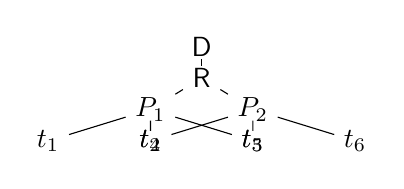
\begin{tikzpicture}[level distance=0.4cm, sibling distance=1.3cm]
        % Database level
        \node {D}
            child {
                node {R}
                child {
                    node {$P_1$}
                    child { node {$t_1$} }
                    child { node {$t_2$} }
                    child { node {$t_3$} }
                }
                child {
                    node {$P_2$}
                    child { node {$t_4$} }
                    child { node {$t_5$} }
                    child { node {$t_6$} }
                }
            };
    \end{tikzpicture}
    \columnbreak
    \begin{itemize}
        \item If T is holding a $S$ on $P_1$, then T is implicitly holding a $S$ on $t_1$, $t_2$, $t_3$
        \item If T is holding a $X$ on $R$, then T is implicitly holding a $X$ on $P_1$, $P_2$, $t_1$, $t_2$, $t_3$, $t_4$, $t_5$, \& $t_6$
    \end{itemize}
\end{multicols}

\subsubsubsection{Multi-granular Locking Protocol}
\begin{itemize}
    \item \textbf{Idea:} Use a new intention lock (I-lock) mode
    \item \textbf{Protocol:} Before acquiring S-lock/X-lock on a data granule G, need to acquire I-locks on granules coarser than G in a top-down manner
    \item \textbf{Example:} Xact $T$ wants to request X-lock on tuple $t_4$
    \begin{itemize}
        \item Must first acquire $I$ locks on D, then R, then $P_2$ before acquiring X-lock on $t_4$
    \end{itemize}
    \item \textbf{Problem:} \textcolor{red}{Limited concurrency} with lock modes I, S, and X
    \item \textbf{Example:} Suppose $T_1$ has a S-lock on $t_4$ $\implies$ $T_1$ has I-locks on D, R \& $P_2$
    \begin{itemize}
        \item If $T_2$ wants to read $P_2$:
        \item[$\triangleright$] its $I$ req on D \& R will be granted, but its $S$ request on $P_2$ will be blocked
    \end{itemize}
\end{itemize}

\subsubsubsection{Multi-granular Locking Protocol | Refined}
\begin{itemize}
    \item Refine \textit{intention lock} idea with IS \& IX lock modes
    \begin{itemize}
        \item[$\triangleright$] \textcolor{blue}{intention shared (IS)}: intent to set S-locks at finer granularity
        \item[$\triangleright$] \textcolor{blue}{intention exclusive (IX)}: intent to set X-locks at finer granularity
    \end{itemize}
    \item \textbf{Lock compatibility matrix:}
    \begin{multicols}{2}
        \begin{center}
            \resizebox{\columnwidth}{!}{
            \begin{tabular}{|c|c|c|c|c|c|}
                \hline
                \rowcolor{lightgray}
                \diagbox[width=6em]{\tiny Lock Requested}{\tiny LockHeld} & \tiny - & \tiny IS & \tiny IX & \tiny S & \tiny X \\
                \hline
                IS & $\checkmark$ & $\checkmark$ & $\checkmark$ & $\checkmark$ & $\times$ \\
                \hline
                IX & $\checkmark$ & $\checkmark$ & $\checkmark$ & $\times$ & $\times$ \\
                \hline
                S & $\checkmark$ & $\checkmark$ & $\times$ & $\checkmark$ & $\times$ \\
                \hline
                X & $\checkmark$ & $\times$ & $\times$ & $\times$ & $\times$ \\
                \hline
            \end{tabular}
            }
        \end{center}
        \item \textcolor{red}{Multi-granular locking protocol:}
        \begin{itemize}
            \item[$\triangleright$] Locks are \underline{acquired} in \textit{top-down order}, \underline{released} in \textit{bottom-up order}
            \item[$\triangleright$] To obtain $S/IS$ lock on node, must already hold $IS/IX$ on parent node
            \item[$\triangleright$] To obtain $X/IX$ lock on node, must already hold $IX$ lock on parent node
        \end{itemize}
    \end{multicols}
\end{itemize}

\subsection{9. Multiversion Concurrency Control}
\begin{itemize}
    \item $W_i(O)$ creates a new ver. of object $O$ |  $R_i(O)$ reads appropriate ver. of $O$
    \item \textbf{Advantages:}
    \begin{itemize}
        \item[$\triangleright$] Read-only Xacts are not blocked by update Xacts
        \item[$\triangleright$] Update Xacts not blocked by read-only Xacts, Read-only Xacts never aborted
    \end{itemize}
    % \item \textbf{Notation:}
    % \begin{itemize}
    %     \item[$\triangleright$] $W_i(x)$ creates a new version of $x$ denoted by $x_i$
    %     \item[$\triangleright$] For each object $x$, its initial version is denoted by $x_0$
    % \end{itemize}
    % \item \textbf{Example:}
    %     \begin{tabular}{|l|l|l|}
    %         \hline
    %         $T_1$ & $T_2$ & Comments \\
    %         \hline
    %         & & $x_0 = 10$, $y_0 = 20$ \\
    %         & $R_2(x)$ & 10 \\
    %         $W_1(y)$ & & $y_1 = 100$ \\
    %         & $R_2(y)$ & ? \\
    %         \hline
    %     \end{tabular}
    % \item In 2PL, $R_2(y)$ will be blocked
    % \item In MVCC:
    % \begin{itemize}
    %     \item[$\triangleright$] $W_1(y)$ creates a new version of $y$ (with a value of 100)
    %     \item[$\triangleright$] $R_2(y)$ is not blocked
    %     \item[$\triangleright$] $R_2(y)$ returns 20 (the value of the version before $W_1(y)$)
    %     \item[$\triangleright$] Read-only Xacts are never blocked/aborted
    % \end{itemize}
\end{itemize}

\begin{itemize}
    \item \textbf{Multiversion Schedules:}
        \begin{itemize} 
            \item If there are multiple versions of an obj $x$, a \textit{read} on $x$ could return \textit{any version}
            \item $\therefore$ interleaved exec could correspond to diff MVS depending on MVCC protocol
        \end{itemize}
    \item \textbf{Multiversion View Equivalence:} $S$ and $S'$, over same set of transactions, are defined to be \textcolor{red}{multiversion view equivalent} ($S \equiv_{mv} S'$) if they have the same set of read-from relationships $\triangleright$ i.e., $R_i(x_j)$ occurs in $S$ iff $R_i(x_j)$ occurs in $S'$
    \item \textbf{Monoversion Schedules:} A multiversion schedule $S$ is called a \textcolor{red}{monoversion schedule} if each read action in $S$ returns the \textit{most recently created object version}
    \item \textbf{Serial Monoversion Schedules:} Monoversion schedule that is \textcolor{red}{also a serial}
\end{itemize} 

% \subsubsubsection{Multiversion Schedules}
% \begin{itemize}
%     \item If there are multiple versions of an object $x$, a \textit{read} on $x$ could return \textit{any version}
%     \item $\therefore$ interleaved exec could correspond to diff MVS depending on MVCC protocol
%     % \item \textbf{Example:} $R_1(x)$, $W_1(x)$, $R_2(x)$, $W_2(y)$, $R_1(y)$, $W_1(z)$
%     % \begin{itemize}
%     %     \item $S_1$: $\textcolor{blue}{R_1(x_0)}$, $\textcolor{blue}{W_1(x_1)}$, $\textcolor{red}{R_2(x_0)}$, $\textcolor{red}{W_2(y_2)}$, $\textcolor{blue}{R_1(y_0)}$, $\textcolor{blue}{W_1(z_1)}$
%     %     \item $S_2$: $\textcolor{blue}{R_1(x_0)}$, $\textcolor{blue}{W_1(x_1)}$, $\textcolor{red}{R_2(x_1)}$, $\textcolor{red}{W_2(y_2)}$, $\textcolor{blue}{R_1(y_2)}$, $\textcolor{blue}{W_1(z_1)}$
%     %     \item $S_3$: $\textcolor{blue}{R_1(x_0)}$, $\textcolor{blue}{W_1(x_1)}$, $\textcolor{red}{R_2(x_1)}$, $\textcolor{red}{W_2(y_2)}$, $\textcolor{blue}{R_1(y_0)}$, $\textcolor{blue}{W_1(z_1)}$
%     %     \item $S_4$: $\textcolor{blue}{R_1(x_0)}$, $\textcolor{blue}{W_1(x_1)}$, $\textcolor{red}{R_2(x_1)}$, $\textcolor{red}{W_2(y_2)}$, $\textcolor{blue}{R_1(y_2)}$, $\textcolor{blue}{W_1(z_1)}$
%     % \end{itemize}
%     % \item \textbf{Notes:}
%     % \begin{itemize}
%     %     \item[$\triangleright$] $R_1(x)$ returns $x_0$
%     %     \item[$\triangleright$] $R_2(x)$ could return $x_0$ or $x_1$
%     %     \item[$\triangleright$] $R_1(y)$ could return $y_0$ or $y_2$
%     % \end{itemize}
% \end{itemize}

% \subsubsubsection{Multiversion View Equivalence}
% \begin{itemize}
%     \item $S$ and $S'$, over same set of transactions, are defined to be \textcolor{red}{multiversion view equivalent} ($S \equiv_{mv} S'$) if they have the same set of read-from relationships
%     \begin{itemize}
%         \item[$\triangleright$] i.e., $R_i(x_j)$ occurs in $S$ iff $R_i(x_j)$ occurs in $S'$
%     \end{itemize}
% \end{itemize}

% \subsubsubsection{Monoversion Schedules}
% \begin{itemize}
%     \item A multiversion schedule $S$ is called a \textcolor{red}{monoversion schedule} if each read action in $S$ returns the \textit{most recently created object version}
%     % \item \textbf{Example:} $\textcolor{blue}{R_1(x)}$, $\textcolor{blue}{W_1(x)}$, $\textcolor{red}{R_2(x)}$, $\textcolor{red}{W_2(y)}$, $\textcolor{blue}{R_1(y)}$, $\textcolor{blue}{W_1(z)}$
%     % \begin{itemize}
%     %     \item $S_1$: $\textcolor{blue}{R_1(x_0)}$, $\textcolor{blue}{W_1(x_1)}$, $\textcolor{red}{R_2(x_0)}$, $\textcolor{red}{W_2(y_2)}$, $\textcolor{blue}{R_1(y_0)}$, $\textcolor{blue}{W_1(z_1)}$
%     %     \item $S_2$: $\textcolor{blue}{R_1(x_0)}$, $\textcolor{blue}{W_1(x_1)}$, $\textcolor{red}{R_2(x_0)}$, $\textcolor{red}{W_2(y_2)}$, $\textcolor{blue}{R_1(y_2)}$, $\textcolor{blue}{W_1(z_1)}$
%     %     \item $S_3$: $\textcolor{blue}{R_1(x_0)}$, $\textcolor{blue}{W_1(x_1)}$, $\textcolor{red}{R_2(x_1)}$, $\textcolor{red}{W_2(y_2)}$, $\textcolor{blue}{R_1(y_0)}$, $\textcolor{blue}{W_1(z_1)}$
%     %     \item $S_4$: $\textcolor{blue}{R_1(x_0)}$, $\textcolor{blue}{W_1(x_1)}$, $\textcolor{red}{R_2(x_1)}$, $\textcolor{red}{W_2(y_2)}$, $\textcolor{blue}{R_1(y_2)}$, $\textcolor{blue}{W_1(z_1)}$
%     % \end{itemize}
%     % \item \textbf{Notes:}
%     % \begin{itemize}
%     %     \item[$\triangleright$] $S_1$ is a monoversion schedule
%     %     \item[$\triangleright$] $S_1$, $S_2$, and $S_3$ are not monoversion schedules
%     % \end{itemize}
% \end{itemize}

% \subsubsubsection{Serial Monoversion Schedules}
% \begin{itemize}
%     \item A monoversion schedule is defined to be a \textcolor{red}{serial monoversion schedule} if it is also a serial schedule
%     % \item \textbf{Example:}
%     % \begin{itemize}
%     %     \item $S_1$: $\textcolor{blue}{R_1(x_0)}$, $\textcolor{blue}{W_1(x_1)}$, $\textcolor{red}{R_2(x_1)}$, $\textcolor{red}{W_2(y_2)}$, $\textcolor{green}{C_1}$, $\textcolor{blue}{R_1(y_2)}$, $\textcolor{blue}{W_1(z_1)}$, $\textcolor{green}{C_1}$
%     %     \item $S_2$: $\textcolor{blue}{R_1(x_0)}$, $\textcolor{blue}{W_1(x_1)}$, $\textcolor{blue}{R_1(y_0)}$, $\textcolor{blue}{W_1(z_1)}$, $\textcolor{green}{C_1}$, $\textcolor{red}{R_2(x_1)}$, $\textcolor{red}{W_2(y_2)}$, $\textcolor{green}{C_2}$
%     % \end{itemize}
%     % \item \textbf{Notes:}
%     % \begin{itemize}
%     %     \item[$\triangleright$] $S_1$ is a non-serial monoversion schedule
%     %     \item[$\triangleright$] $S_2$ is a serial monoversion schedule
%     % \end{itemize}
% \end{itemize}

\subsubsubsection{Multiversion View Serializability}
\begin{itemize}
    \item A multiversion schedule $S$ is defined to be \textcolor{red}{multiversion view serializable schedule (MVSS)} if there exists a \textcolor{red}{serial monoversion schedule} (over the same set of Xacts) that is multiversion view equivalent to $S$
    \item \hl{\textbf{Theorem 1:} A VSS is also a multiversion VSS (MVSS)} not necessarily vice versa
    % \item \textbf{Example:}
    % \begin{itemize}
    %     \item $T_1$: $\textcolor{blue}{R_1(x_0)}$, $\textcolor{blue}{R_1(y_0)}$, $\textcolor{green}{Commit_1}$
    %     \item $T_2$: $\textcolor{red}{W_2(x_2)}$, $\textcolor{red}{W_2(y_2)}$, $\textcolor{green}{Commit_2}$
    %     \item The above schedule is multiversion view equivalent to the serial monoversion schedule $(T_1, T_2)$
    %     \item However, the schedule is not a valid monoversion schedule (due to $W_2(x_2)$ \& $R_1(y_0)$) and is therefore not VSS
    % \end{itemize}
\end{itemize}

\subsubsubsection{Testing for MVSS}
\begin{itemize}
    \item We can generalize the VSG approach (used for testing VSS) to test for MVSS
    \item A \textcolor{red}{multiversion view serializability graph} for a schedule $S$ (denoted by \textcolor{red}{$MVSG(S)$}) is a directed graph $MVSG(S) = (V,E)$ such that the nodes $V$ represent Xacts \& the edges $E$ represent precedence relations among Xacts:
    \begin{itemize}
        \item[(a)] If $T_j$ reads from $T_i$, then $(T_i, T_j) \in E$
        \item[(c)] If $T_j$ read some object $O$ from $T_i$ \& $T_l$ update object $O$, then either $(T_i, T_l) \in E$ or $(T_l, T_j) \in E$
    \end{itemize}
    \item Due to (c), there could be multiple MVSG(S) corresponding to S
    \item Notice that (b) from VSS is missing, as that is for \underline{final write}
    \item \hl{\textbf{Theorem 2:} S is MVSS iff $\exists$ some MVSG(S) corresponding to S that is acyclic}
\end{itemize}

% \subsubsubsection{Concurrent Transactions}
% \begin{itemize}
%     \item Two Xacts $T$ and $T'$ are defined to be \textcolor{red}{concurrent} if they overlap
%     \begin{itemize}
%         \item[$\triangleright$] i.e., $[start(T),commit(T)] \cap [start(T'),commit(T')] \neq \emptyset$
%     \end{itemize}
%         \tiny
%         \begin{tabular}{|c|c|c|c|}
%             \hline
%             Timestamp & $T_1$ & $T_2$ & $T_3$ \\
%             \hline
%             1 & \cellcolor{red}{$R_1(B)$} & & \\
%             2 & & & \\
%             3 & \cellcolor{red}{$W_1(B)$} & & \\
%             4 & \cellcolor{red}{$Commit_1$} & & \\
%             5 & & \cellcolor{cyan}{$R_2(B)$} & \\
%             6 & & \cellcolor{cyan}{$W_2(A)$} & \\
%             7 & & & \cellcolor{teal}{$R_3(A)$} \\
%             8 & & & \cellcolor{teal}{$R_3(B)$} \\
%             9 & & & \cellcolor{teal}{$Commit_3$} \\
%             10 & & \cellcolor{cyan}{$Commit_2$} & \\
%             \hline
%         \end{tabular}
% \end{itemize}

\textbf{Concurrent Txn:} Two Xacts $T$ and $T'$ are defined to be \textcolor{red}{concurrent} if they overlap $\rightarrow$ i.e., $[start(T),commit(T)] \cap [start(T'),commit(T')] \neq \emptyset$ \\ 
\textbf{Snapshot Isolation (SI)} | break the “Concurrent Update Property” to not be SI
\begin{itemize}
    \item Each Xact $T$ sees a snapshot of DB that consists of updates by Xacts that committed before $T$ starts and each Xact $T$ associated with 2 timestamps:
    \begin{itemize}
        \item[$\triangleright$] \textcolor{blue}{start(T)}: the time that $T$ starts | \textcolor{blue}{commit(T)}: the time that $T$ commits
    \end{itemize}
    \item $W_i(O)$ creates a version of $O$ denoted by $O_i$
    \item $O_i$ \textcolor{blue}{more recent/newer} version compared to $O_j$ if $commit(T_i) > commit(T_j)$
    \item $R_i(O)$ reads either its own update (if $W_i(O)$ precedes $R_i(O)$) or the latest version of $O$ that is created by a Xact that committed before $T_i$ started; i.e., If $R_i(O)$ returns $O_j$, then:
    \begin{enumerate}
        \item Either $j = i$ if $W_i(O)$ precedes $R_i(O)$;
        \item Or $commit(T_j) < start(T_i)$, and
        \begin{enumerate}
            \item For every Xact $T_k$, $k \neq j$, that has created a version $O_k$ of $O$, if $commit(T_k) < start(T_i)$, then $commit(T_k) < commit(T_j)$
        \end{enumerate}
    \end{enumerate}
    \item \textbf{Concurrent Update Property:} If multiple concurrent Xacts update same object, only 1 of the Xacts is allowed to commit, if not, schedule may not be serializable
    % \begin{itemize}
    %     \item[$\triangleright$] \textbf{Example:} Consider the following schedule $S$:
    %     \begin{flushleft}
    %         $T_1$: $\textcolor{red}{R_1(x_0)}$ \hspace{2em} $\textcolor{red}{W_1(x_1)}$ \hspace{8em} $\textcolor{red}{Commit_1}$ \\
    %         $T_2$: \hspace{2em} $\textcolor{blue}{R_2(x_0)}$ \hspace{4em} $\textcolor{blue}{W_2(x_2)}$ $\textcolor{blue}{Commit_2}$
    %     \end{flushleft}
    %     \item[$\triangleright$] $S$ is not serializable!
    % \end{itemize}
    \item Two approaches to enforce the concurrent update property:
    \begin{itemize}
        \item[$\triangleright$] First Committer Wins (FCW) Rule OR First Updater Wins (FUW) Rule
    \end{itemize}
\end{itemize}

\subsubsubsection{First Committer Wins (FCW) Rule}
\begin{itemize}
    \item Before committing a Xact $T$, the system checks if there exists a committed concurrent Xact $T'$ that has updated some object that $T$ has also updated
    \item If $T'$ exists, then $T$ aborts
\end{itemize}

\subsubsubsection{First Updater Wins (FUW) Rule}
\begin{itemize}
    \item Whenever a Xact $T$ needs to update an object $O$, $T$ requests for a X-lock on $O$
    \item If the X-lock is not held by any concurrent Xact, then
    \begin{itemize}
        \item[$\triangleright$] $T$ is granted the X-lock on $O$
        \item[$\triangleright$] If $O$ has been updated by any committed concurrent Xact, then $T$ aborts
        \item[$\triangleright$] Otherwise, $T$ proceeds with its execution
    \end{itemize}
    \item Otherwise, if the X-lock is being held by some concurrent Xact $T'$, then $T$ aborts or commits
    \begin{itemize}
        \item[$\triangleright$] If $T'$ aborts, then
        \begin{itemize}
            \item[$\bullet$] Assume that $T$ is granted the X-lock on $O$
            \item[$\bullet$] If $O$ has been updated by any concurrent Xact, then $T$ aborts
            \item[$\bullet$] Otherwise, $T$ proceeds with its execution
        \end{itemize}
        \item[$\triangleright$] If $T'$ commits, then $T$ is aborted
    \end{itemize}
    \item When a Xact commits/aborts, it releases its X-lock(s)
\end{itemize}

\textbf{Garbage Collection:}  A version $O_i$ of object $O$ may be deleted if there exists a newer version $O_j$ (i.e., $commit(T_i) < commit(T_j)$) such that for every active Xact $T_k$ that started after the commit of $T_i$ (i.e., $commit(T_i) < start(T_k)$), we have $commit(T_j) < start(T_k)$
% \begin{itemize}
    % \item \textbf{Example:}
    % \begin{center}
    %     \includegraphics*[width=8.5cm, height=1.5cm]{images/garbage.png}
    % \end{center}
    % \item Active transactions: $T_3$ \& $T_5$
    % \item Versions that can be deleted: $x_4$ \& $x_5$
% \end{itemize}

\subsubsubsection{Snapshot Isolation Tradeoffs}
\begin{itemize}
    \item Performance of SI often similar to \textit{Read Committed}
    \item Unlike Read Committed, SI does not suffer from lost update/unrepeatable read
    \item But SI is vulnerable to some non-serializable executions
    \begin{itemize}
        \item[$\triangleright$] Write Skew Anomaly OR Read-Only Transaction Anomaly
    \end{itemize}
    \item Snapshot isolation does not guarantee serializability
\end{itemize}

\begin{multicols}{2}
    \textbf{Write Skew Anomaly}
        \tiny
        \begin{tabular}{|c|c|}
            \hline
            $T_1$ & $T_2$ \\
            \hline
            $\textcolor{red}{R_1(x_0)}$ & \\
            $\textcolor{red}{R_1(y_0)}$ & \\
            & $\textcolor{blue}{R_2(x_0)}$ \\
            & $\textcolor{blue}{R_2(y_0)}$ \\
            $\textcolor{red}{W_1(x_1)}$ & \\
            $\textcolor{red}{Commit_1}$ & \\
            & $\textcolor{blue}{W_2(y_2)}$ \\
            & $\textcolor{blue}{Commit_2}$ \\
            \hline
        \end{tabular} \\
       The above is a SI schedule that is not a MVSS \\
    \columnbreak
    \textbf{\scriptsize{Read-Only Transaction Anomaly}}
    \tiny
        \begin{tabular}{|c|c|c|}
            \hline
            $T_1$ & $T_2$ & $T_3$ \\
            \hline
            $\textcolor{red}{R_1(y_0)}$ & & \\
            & $\textcolor{blue}{R_2(x_0)}$ & \\
            $\textcolor{red}{W_1(y_1)}$ & & \\
            $\textcolor{red}{Commit_1}$ & & \\
            & $\textcolor{blue}{R_2(y_0)}$ & \\
            & $\textcolor{blue}{W_2(x_2)}$ & \\
            & $\textcolor{blue}{Commit_2}$ & \\
            & & $\textcolor{teal}{R_3(x_0)}$ \\
            & & $\textcolor{teal}{R_3(y_1)}$ \\
            & & $\textcolor{teal}{Commit_3}$ \\
            \hline
        \end{tabular}
    The above is a SI schedule that is not a MVSS
\end{multicols}

\subsubsubsection{Serializable Snapshot Isolation (SSI) Protocol}
\begin{itemize}
    \item A schedule $S$ is a \textcolor{red}{serializable snapshot isolation (SSI) schedule} if $S$ is produced by the snapshot isolation protocol (i.e., $S$ is a SI schedule) and $S$ is MVSS
\end{itemize}


\subsection{10. Crash Recovery}
\begin{itemize}
    \item \textbf{Recovery Manager} guarantees atomicity and durability of transactions
    \begin{itemize}
        \item \textcolor{blue}{\textbf{Commit(T)}} - install T's updated pages into database
        \item \textcolor{blue}{\textbf{Abort(T)}} - restore all data that T updated to their prior values
        \item \textcolor{blue}{\textbf{Restart}} - recover database to a consistent state from system failure
        \begin{itemize} % Nested itemize for Restart sub-points
            \item[$\triangleright$] abort all active Xacts at the time of system failure
            \item[$\triangleright$] installs updates of all committed Xacts that were not installed in the database before the failure
        \end{itemize}
    \end{itemize}
\end{itemize}

\subsubsubsection{Interaction of Recovery \& Buffer Managers} % Added subsubsubsection
\begin{itemize}
    \fontsize{5.9pt}{7pt}\selectfont
    \item \textcolor{red}{Steal policy}: allows dirty pages updated by $T$ to be replaced from buffer pool before $T$ commits
    \item \textcolor{red}{Force policy}: requires all dirty pages updated by $T$ to be written to disk when $T$ commits \\ 
        \vspace{0.5ex}
        \noindent
        \begin{minipage}[t]{0.61\linewidth}
            \begin{tabular}{|c|c|c|}
                \rowcolor{lightgray}
                \hline
                    & \textbf{Force} & \textbf{No-force} \\
                \hline
                \textbf{Steal} & undo \& no redo & \textcolor{blue}{undo \& redo} \\
                \hline
                \textbf{No-steal} & no undo \& no redo & no undo \& redo \\
                \hline
            \end{tabular}
        \end{minipage}%
        \begin{minipage}[t]{0.39\linewidth}
            \vspace*{-10pt}
            \begin{itemize}
                \item[$\triangleright$] No-steal policy $\implies$ no undo
                \item[$\triangleright$] Force policy $\implies$ no redo
            \end{itemize}
        \end{minipage}
\end{itemize}

\subsubsubsection{Log-based Database Recovery}
\begin{itemize}
    \item \textcolor{red}{Log} (aka trail/journal): history of actions executed by DBMS
    \begin{itemize}
        \item Contains a log record for each write, commit, \& abort
    \end{itemize}
    \item Log is stored as a sequential file of records in stable storage
    \item Log is stored in \textcolor{red}{stable storage} (storage that can survive crashes \& media failures)
    \begin{itemize}
        \item Implemented by maintaining multiple copies of information (possibly at different locations) on non-volatile storage devices
    \end{itemize}
\end{itemize}

\textbf{Log Sequence Number (LSN):} monotonically increasing. Recently created log records are buffered in the main memory before they are flushed (i.e., written) to the log file on disk. Recovery manager maintains a metadata known as \textcolor{red}{flushedLSN} to keep track of the LSN of the last log record that has been flushed to disk 
% \begin{itemize}
%     \item Log record has a \textit{unique identifier} called \textbf{Log Sequence Number (LSN)}
%     \item LSNs are \textit{monotonically increasing}: the LSN of an earlier $<$ later log record
%     \item Recently created log records are buffered in the main memory before they are flushed (i.e., written) to the log file on disk
%     \item Recovery manager maintains a metadata known as \textcolor{red}{flushedLSN} to keep track of the LSN of the last log record that has been flushed to disk
%     \item Each data page $P$ has a metadata named \textcolor{red}{pageLSN} that records the LSN of the most recent log record created for $P$
% \end{itemize}

\textbf{ARIES Recovery Algorithm:} \textcolor{red}{steal, no-force} approach, assumes strict 2PL

\subsubsubsection{Recovery-related Structures}
\includegraphics*[width=8.5cm, height=2.8cm]{images/xactprocessing.png}

% \begin{itemize}
%     \item \textcolor{blue}{Log file}
%     \item \textcolor{blue}{Transaction table (TT)}: One entry for each \textcolor{red}{active Xact}, each entry contains:
%     \begin{itemize}
%         \item[$\star$] XactID: Transaction identifier
%         \item[$\star$] \textcolor{red}{lastLSN}: LSN of the most recent log record for this Xact
%         \item[$\star$] Xact status (C or U) | C = Xact has committed |  Xact has not committed
%     \end{itemize}
%     \item \textcolor{blue}{Dirty page table (DPT)}: One entry for each \textcolor{red}{dirty page} in buffer pool, contains:
%     \begin{itemize}
%         \item[$\star$] pageID: page ID of dirty page
%         \item[$\star$] \textcolor{red}{recLSN}: LSN of earliest log record for an update that dirtied the page
%     \end{itemize}
% \end{itemize}

    % \begin{tabular}{|p{0.15\linewidth}|p{0.84\linewidth}|}
    % \hline
    % \rowcolor{lightgray}
    % \textbf{Field} & \textbf{Description} \\
    % \hline
    % LSN & Each log record has a unique Log Sequence Number (LSN) \\
    % \hline
    % XactID & Identifier of transaction that created log record \\
    % \hline
    % type & $\in \{$update, compensation, commit, abort, end, checkpoint$\}$ \\
    % \hline
    % pageID & Identifier of page being updated \\
    % \hline
    % length, offset & Number of bytes modified on page; offset = starting byte offset of modification on page \\
    % \hline
    % recLSN & LSN of earliest update log record for a dirty page \\
    % \hline
    % lastLSN & LSN of most recent log record for a transaction \\
    % \hline
    % status & Status of transaction (Uncommitted or Committed) \\
    % \hline
    % prevLSN & All the log records for a transaction are backward linked via prevLSN \\
    % \hline
    % \end{tabular}

\subsubsubsection{Normal Transaction Processing}
\textcolor{blue}{\textbf{Updating Xact Table (transID, lastLSN, status)}}
\begin{itemize}
    \item When \textbf{first} log record is created for $T$, create a new entry for $T$ with status = U
    \item When \textbf{new} log record $r$ created for $T$, update \texttt{lastLSN} for $T$ to be $r$'s LSN
    \item If Xact $T$ commits, update \texttt{status} for $T$'s entry to be C
    \item When an end log record is generated for Xact $T$, remove $T$'s entry
\end{itemize}

\textcolor{blue}{\textbf{Updating Dirty Page Table (pageID, recLSN)}}
\begin{itemize}
    \item When a page $P$ in buffer pool is updated \& DPT has no entry for $P$, create a new table entry for $P$ with recLSN = LSN of \textit{log record corresponding to update}
    \item When a dirtied page $P$ in buffer pool is \textit{flushed to disk}, remove entry for $P$
\end{itemize}

\subsubsubsection{Types of log records}
\begin{itemize}
    \item All log records have the following information:
    \begin{enumerate}
        \item type of log record (e.g., update, commit, abort),
        \item identifier of Xact, and \texttt{prevLSN} (LSN of previous log record for same Xact)
    \end{enumerate}
    \item \textcolor{red}{\textbf{Update log record}}: created after updating page $P$, update pageLSN = LSN of $r$
    \begin{itemize}
        \item Additional fields in ULR: pageID, offset, length, before-image, after-image
        % \begin{itemize}
        %     \item[$\star$] \textbf{pageID}: identifier of page being updated
        %     \item[$\star$] \textbf{offset}: byte offset within page indicating the beginning of updated portion
        %     \item[$\star$] \textbf{length}: number of bytes for updated portion of data page
        %     \item[$\star$] \textbf{before-image}: value of the changed bytes before update
        %     \item[$\star$] \textbf{after-image}: value of the changed bytes after update
        % \end{itemize}
    \end{itemize}
    \item \textcolor{red}{\textbf{Compensation log record (CLR)}}
    \begin{itemize}
        \item When update described by an ULR is undone, create a CLR
        \item Additional fields in CLR:
        \begin{itemize}
            \item[$\star$] \textcolor{blue}{page ID}, \textcolor{blue}{undoNextLSN} = LSN of next log record to be undone (prevLSN in ULR), \textcolor{blue}{action taken to undo update} (length/offset/before-image)
        \end{itemize}
    \end{itemize}
    \item \textcolor{red}{\textbf{Commit log record}}: created when Xact is committed
    \item \textcolor{red}{\textbf{Abort log record}}: created when Xact is aborted, undo initiated for this Xact
    \item \textcolor{red}{\textbf{End log record}}: once the additional follow-up processing initiated by a aborted/committed Xact $T$ has completed, create an end log record for $T$
    \item \textcolor{red}{\textbf{Checkpoint log record}}
    % \begin{itemize}
    %     \item To be discussed later
    % \end{itemize}
    \item \textcolor{blue}{\textbf{Update log records}} \& \textcolor{blue}{\textbf{CLRs}} are classified as \textcolor{red}{redoable log records}
\end{itemize}

\textbf{Implementing Abort:} Undo all updates by Xact to database pages
\begin{itemize}
    \item \textcolor{red}{\textbf{Write-ahead logging (WAL) protocol}} \\
    Do not flush an uncommitted update to the database until the log record containing its before-image has been flushed to the log
    \begin{itemize}
        \item[$\star$] Before flushing a \textbf{database page} $P$ to disk, ensure that all the log records up to the log record corresponding to \textbf{$P$'s pageLSN} have been flushed to disk
        \item[$\star$] Ensure that $P$'s \textcolor{blue}{pageLSN} $\leq$ \textcolor{blue}{flushedLSN} before $P$ is flushed to disk
    \end{itemize}
    \item For each log record of Xact in reverse order, restore its before-image to undo all
    \item \textbf{How to efficiently retrieve Xact's log records in reverse order?}
    \begin{itemize}
        \item \textcolor{red}{Xact Table (TT)} - maintains one entry for each active Xact
        \item Each TT entry stores the LSN of most recent log record for Xact (\textcolor{red}{lastLSN})
        \item Use \textbf{lastLSN} to retrieve the most recent log record for Xact; the other log records for Xact are retrieved via the \textbf{prevLSN} of each retrieved log record
    \end{itemize}
    \item \textcolor{red}{\textbf{Logging Changes During Undo:}} Changes made to database while undoing a Xact are also logged (using \textcolor{blue}{compensation log records}) to ensure that an action is not repeated in the event of repeated undos
\end{itemize}

\textbf{Implementing Commit:} Need to ensure that all the updates of Xact must be in stable storage (database or log) before Xact is committed
\begin{itemize}
    \item \textcolor{red}{\textbf{Force-at-commit protocol}:} Do not commit a Xact until the after-images of all its updated records are in stable storage (database or log)
    \item Write a commit log record for Xact, then flush all the log records for Xact to disk
    \item \underline{Considered committed} if its commit log record has been written to stable storage
\end{itemize}

\textbf{Implementing Restart} Recovery from system crashes consists of three phases:
\begin{itemize}
    \item \textcolor{red}{\textbf{Repeat history on redo}}: During restart following a crash, first restore system to state before crash, then undo actions of Xacts that are active at the time of crash
    \item \textcolor{red}{\textbf{Log changes during undo}}: Each undone action is logged with a CLR
    \begin{enumerate}
        \item \textcolor{blue}{Analysis}: identifies dirtied buffer pool pages \& \underline{active Xacts} at time of crash
        \item \textcolor{blue}{Redo}: redo actions to restore database state to what it was at time of crash
        \item \textcolor{blue}{Undo}: undo actions of Xacts that did not commit
    \end{enumerate}
\end{itemize}

\textbf{Analysis Phase | Fuzzy checkpointing highlihighted in} \sethlcolor{green}\hl{green}\sethlcolor{yellow}
\begin{itemize}
    \item \sethlcolor{green}\hl{Retrieve \textbf{begin\_checkpoint log record} (BCPLR) identified by the \textbf{master record}}\sethlcolor{yellow}
    \item \sethlcolor{green}\hl{Retrieve \textbf{end\_checkpoint log record} (ECPLR) corresponding to BCPLR}\sethlcolor{yellow}
    \begin{itemize}
        \item \sethlcolor{green}\hl{For simplicity, assume that there are no log records between BCPLR \& ECPLR (i.e., ECPLR is the next log record after BCPLR)}\sethlcolor{yellow}
    \end{itemize}
    \item Initialize \textcolor{blue}{(DPT)} \& \textcolor{blue}{Xact table (TT)} to be empty | \sethlcolor{green}\hl{using ECPLR's contents}\sethlcolor{yellow}
    \item Scan the log in forward direction (\sethlcolor{green}\hl{starting from  ECPLR}\sethlcolor{yellow}) to process each \textbf{log record r} (for \textbf{Xact T}):
    \begin{itemize}
        \item If $r$ is an \textcolor{blue}{end log record} $\rightarrow$ Remove $T$ from TT
        \item Else
        \begin{itemize}
            \item[$\star$] Add entry in TT for $T$ if not in TT, Update \textcolor{blue}{lastLSN} of entry to be $r$'s LSN
            \item[$\star$] Update \textcolor{blue}{status} of entry to C if $r$ is a commit log record
        \end{itemize}
        \item If ($r$ is a redoable log record for page $P$) \& ($P$ is not in DPT), then
        \begin{itemize}
            \item[$\star$] Create an entry for $P$ in DPT with pageID of entry = $P$'s pageID and recLSN of entry = $r$'s LSN
        \end{itemize}
    \end{itemize}
    \item At the end of \textcolor{red}{Analysis phase}:
    \begin{itemize}
        \item[$\triangleright$] \textcolor{blue}{Xact table} = list of all active Xacts (with status = U) at time of crash
        \item[$\triangleright$] \textcolor{blue}{dirty page table} = superset of dirty pages at time of crash
    \end{itemize}
\end{itemize}

\textbf{Redo Phase | Fuzzy checkpointing highlihighted in} \sethlcolor{green}\hl{green}\sethlcolor{yellow}
\begin{itemize}
    \item \textcolor{red}{RedoLSN} = smallest recLSN among all dirty pages in DPT
    \item Let $r$ be the log record with LSN = RedoLSN
    \item Scan the log in forward direction starting from $r$
    \item If ($r$ is an update log record) or ($r$ is a CLR) then | \sethlcolor{green}\hl{If (r is a redoable record) and (condition C is false) then}\sethlcolor{yellow} 
    \begin{itemize}
        \item Fetch page $P$ that is associated with $r$
        \item If ($P$'s pageLSN $<$ $r$'s LSN) then
        \begin{itemize}
            \item[$\star$] Reapply logged action in $r$ to $P$, Update $P$'s pageLSN = $r$'s LSN
        \end{itemize}
        \item \sethlcolor{green}\hl{Else: Update P's entry in DPT: recLSN = P's pageLSN + 1}\sethlcolor{yellow}
    \end{itemize}
    \item At the end of Redo Phase,
    \begin{itemize}
        \item[$\triangleright$] Create end log records for Xacts with status = C in Xact Table \& remove their entries from Xact Table $\Rightarrow$ System is restored to state at time of crash
    \end{itemize}
\end{itemize}

\textbf{Undo Phase | Fuzzy checkpointing highlihighted in} \sethlcolor{green}\hl{green}\sethlcolor{yellow}
\begin{itemize}
    \item \textbf{Goal}: abort active Xacts at time of crash (\textcolor{red}{loser Xacts})
    \begin{itemize}
        \item[$\triangleright$] Abort loser Xacts by undoing their actions in \textit{reverse order}
    \end{itemize}
    \item Initialize $L$ = set of lastLSNs (with status = U) from TT
    \item Repeat until $L$ becomes empty
    \begin{itemize}
        \item delete the largest LSN from $L$
        \item let $r$ be the log record corresponding to the deleted LSN
        \item if $r$ is an \textcolor{red}{update log record} for Xact $T$ on page $P$ then
        \begin{itemize}
            \item[$\star$] create a CLR $r_2$ for $T$: $r_2$'s undoNextLSN = $r$'s prevLSN
            \item[$\star$] update $T$'s entry in TT: lastLSN = $r_2$'s LSN
            \item[$\star$] \sethlcolor{green}\hl{create a DPT entry for P (with recLSN = $r_2$'s LSN if P not in DPT)}\sethlcolor{yellow}
            \item[$\star$] undo the logged action on page $P$
            \item[$\star$] update $P$'s pageLSN = $r_2$'s LSN
            \item[$\star$] \textbf{Update-L-and-TT}($r$'s prevLSN)
        \end{itemize}
        \item else if $r$ is a CLR for Xact $T$ then
        \begin{itemize}
            \item[$\star$] \textbf{Update-L-and-TT}($r$'s undoNextLSN)
        \end{itemize}
        \item else if $r$ is abort log record for Xact $T$ then \textbf{Update-L-and-TT}($r$'s prevLSN)
    \end{itemize}
    \item \fbox{%
        \begin{minipage}{0.93\linewidth}
        \textbf{Update-L-and-TT} (lsn):  if lsn is not null then add lsn to $L$
        \begin{itemize}
            \item else create an end log record for $T$ \& remove $T$'s entry from TT
        \end{itemize}
        \end{minipage}
    }
\end{itemize}

\textbf{Simple Checkpointing}
\fbox{%
    \begin{minipage}{0.95\linewidth}
    \begin{enumerate}
        \item Stop accepting any new update, commit, \& abort operations
        \item Wait till all active update, commit, \& abort operations have finished
        \item Flush all dirty pages in buffer
        \item Write a \textcolor{red}{checkpoint log record} containing \textcolor{blue}{Xact table}
        \item Resume accepting new update, commit, \& abort operations
    \end{enumerate}
    \end{minipage}
}

\begin{itemize}
    \item During restart recovery, \textit{Analysis} begins with latest \textcolor{red}{checkpoint log record} (CPLR)
    \begin{itemize}
        \item[$\triangleright$] Initialize \textcolor{blue}{Xact table} with CPLR's Xact table and \textcolor{blue}{dirty page table} to be empty
    \end{itemize}
\end{itemize}

\textbf{Fuzzy Checkpointing in ARIES}
\fbox{%
    \begin{minipage}{0.95\linewidth}
    \begin{enumerate}
        \item Let DPT$^*$ be the \textcolor{blue}{dirty page table} \& TT$^*$ be the \textcolor{blue}{Xact table}
        \item Write a \textcolor{red}{begin\_checkpoint log record}
        \item Write a \textcolor{red}{end\_checkpoint log record} containing DPT$^*$ \& TT$^*$
        \item Write a special master record containing the LSN of the \textcolor{red}{begin\_checkpoint log record} to a known place on stable storage
    \end{enumerate}
    \end{minipage}
}

\begin{itemize}
    \item During restart recovery, \textit{Analysis} starts with the \textcolor{red}{begin\_checkpoint log record} (BCPLR) identified by the \textcolor{red}{master record}
    \begin{itemize}
        \item[$\triangleright$] Let ECPLR = \textcolor{red}{end\_checkpoint log record} (ECPLR) corresponding to BCPLR
        \item[$\triangleright$] Assume that there are no log records between BCPLR \& ECPLR
        \item[$\triangleright$] Initialize \textcolor{blue}{Xact table} with ECPLR's Xact table and \textcolor{blue}{DPT} with ECPLR's DPT
    \end{itemize}
\end{itemize}



\end{multicols*}
\end{document}